\chapter{测度与分析}
\label{chap:mathematical-analysis}

第~\ref{chap:sets-functions-and-proofs}章建立对象与条件的语言，第~\ref{chap:combinatorics}章
研究有限选择与计算。本章转向它们留下的无限过程：部分和不断延长，递推持续更新，
一个函数在连续区域上累计，或者一列近似函数逐渐提高精度。有限步骤中的规则能否
保留到极限，取决于比较对象的结构、采用的误差尺度及可核对的控制条件。

本章面向已经学过基础分析、线性代数、概率与组合数学的理工科本科毕业生。
熟悉的极限、求导与积分按用途回顾，把主要解释放在一般空间、测度与极限交换上。
集合的距离与权重是共同基础：距离说明点如何接近，测度说明范围占多少贡献。
序列据此讨论极限、累计与迭代保证；固定一个函数时，局部变化和整体累计承担不同任务。
当函数本身随索引变化，还要判断连续性、导数和积分究竟能否保留。
这条路线把集合、点列、单函数和函数列连起来，也使“有极限”与“可以交换运算”分开。

\section{集合的距离、权重与可测范围}
\label{sec:analysis-set-structures}

第~\ref{chap:sets-functions-and-proofs}章已经给出集合、映射和等价关系。现在同一个集合
还可以承担两项不同的任务：判断两个点是否接近，以及累计一个范围内的贡献。
前一任务需要距离，后一任务需要为集合分配权重。距离确定邻域，可测集合族确定哪些
范围允许赋权；两者可以相容，却不能互相代替。

\subsection{度量与邻域}

实数可以用绝对值之差比较，但一个状态也可能是向量、一张函数或一组概率权重。
此时先要指定什么差异算大、什么差异算小。度量把这种比较归纳为三条规则：
零距离应能辨认同一个对象，比较不分先后，绕经第三个点不会比直接比较更短。
\begin{definition}[度量与度量空间]
\label{def:analysis-metric-space}
集合$X$上的\term{度量}（metric）是函数$d:X\times X\to[0,\infty)$，满足对任意$x,y,z\in X$，
\[
  \begin{aligned}
    d(x,y)=0&\Longleftrightarrow x=y,\\
    d(x,y)&=d(y,x),\\
    d(x,z)&\leq d(x,y)+d(y,z).
  \end{aligned}
\]
带有度量的集合$(X,d)$称为\term{度量空间}（metric space）。
\end{definition}
欧氏空间使用$d(\bm{x},\bm{y})=\lVert\bm{x}-\bm{y}\rVert_2$；有限集合可以使用离散度量$d(x,y)=\mathbb{I}\{x\neq y\}$。同一个集合选择不同度量，可能改变何谓收敛以及函数是否连续；不过，有些度量只改变数值尺度，例如$d$与$2d$具有相同的收敛序列和连续映射。不能仅凭距离公式不同就断言这些性质不同。

\begin{definition}[开球]
\label{def:analysis-open-ball}
在度量空间$(X,d)$中，以$x\in X$为中心、半径$r>0$的开球记为
$B(x,r)=\{y\in X:d(x,y)<r\}$。
\end{definition}

开球把“离一个点足够近”写成集合。若$V\subseteq X$包含某个$B(x,r)$，就称
$V$是$x$的邻域；邻域本身不必是开集。由这些邻域还可以判断一个范围是否包含
其中每个点附近的点。

\begin{definition}[开集与闭集]
\label{def:analysis-open-closed-sets}
在度量空间$(X,d)$中，集合$U\subseteq X$若对每个$x\in U$都存在$r>0$使$B(x,r)\subseteq U$，就称为
\term{开集}（open set）；集合$C\subseteq X$若其补集$X\setminus C$为开集，就称为
\term{闭集}（closed set）。
\end{definition}

开闭性总是相对于当前空间而言。例如$[0,1/2)$在$\mathbb R$中不是开集，
但在子空间$X=[0,1]$中是开集：此时开球是实轴开区间与$X$的交，
$0$的一个小球不必包含负数。全集$X$和空集既开又闭；“不是开集”也不等于
“就是闭集”，实轴上的$[0,1)$便两者都不是。

同一集合上的距离选择也应随比较任务变化。在$\mathbb R$上，通常距离
$d_1(x,y)=|x-y|$把数值相近的状态看作接近，离散距离
$d_2(x,y)=\mathbb I\{x\neq y\}$则只区分相同与不同。
点$0$的$d_1$小球是区间，而半径小于$1$的$d_2$球只有$\{0\}$。
在有限状态的概率向量$\bm p,\bm q$之间，$\sum_i|p_i-q_i|$比较的是整组
权重的差异；在有界函数$f,g:S\to\mathbb R$之间，
$\sup_{x\in S}|f(x)-g(x)|$比较的是所有输入处的最大误差。
后两种距离的点分别是概率向量和函数，不能用一个未指定坐标的实数绝对值代替。
后文会用$1/n$和恒等映射具体核对$d_1,d_2$对收敛、连续性的不同判断。

有时比较规则只能看到对象的一部分，因而会把两个不同对象判为零距离。例如在
$\mathbb R^2$中只比较第一个坐标，$d(\bm x,\bm y)=|x_1-y_1|$仍保留对称性和
三角不等式，却无法区分$(0,0)$与$(0,1)$。后面的样本函数距离和半正定二次型
都需要表达这种分辨力有限的比较。
\begin{definition}[伪距离]
\label{def:analysis-pseudometric}
集合$X$上的\term{伪距离}（pseudometric，也称伪度量）是函数
$d:X\times X\to[0,\infty)$，对所有$x,y,z\in X$满足
\[
 d(x,x)=0,\qquad d(x,y)=d(y,x),\qquad d(x,z)\leq d(x,y)+d(y,z).
\]
它允许$x\neq y$时仍有$d(x,y)=0$；若进一步要求零距离蕴含$x=y$，就得到度量。
\end{definition}
零距离并不意味着原始对象相等。若任务本来就不区分这些对象，可以把它们合并：
定义$x\sim y$当且仅当$d(x,y)=0$。自反性、对称性及三角不等式分别保证这是一项
等价关系。在商集$X/{\sim}=\{[x]:x\in X\}$上定义
\begin{equation}
 \bar d([x],[y])=d(x,y).
\label{eq:analysis-quotient-metric}
\end{equation}
这一定义必须不依赖代表元。若$x\sim x'$且$y\sim y'$，则
$d(x,y)\leq d(x,x')+d(x',y')+d(y',y)=d(x',y')$；交换两对点又得反向不等式，
故距离相等。其余度量条件直接继承，而且$\bar d([x],[y])=0$恰好等价于
$[x]=[y]$，所以商集确实成为度量空间。

在只看第一坐标的例子中，$[(a,b)]=\{(a,t):t\in\mathbb R\}$是一条竖直直线；
商空间中的点是这些直线，两点距离为第一坐标之差的绝对值。原空间丢失的第二坐标
没有被恢复，而是被明确排除在比较对象之外。
第~\ref{sec:analysis-function-convergence-essential-bounds}节中的函数等价类会回用这一做法。

\subsection{测度与可测集}
\subsubsection{可测集合与赋权}

前文的\emph{度量}$d(x,y)$比较两个点相距多远，此处的\emph{测度}$\mu(A)$描述
整个集合$A$占多少权重。两者处理不同对象，并不存在从距离公式直接得到唯一测度的
通用规则。例如$X=\{a,b\}$可以固定离散度量$d(a,b)=1$，却分别使用计数权重
$(1,1)$、非均匀权重$(1,2)$，或归一化后的概率权重$(1/3,2/3)$。
点列的收敛不因此改变，函数的积分却随权重改变。
表~\ref{tab:analysis-metric-measure-integral}把这几个对象分开。

\begin{table}[htbp]
 \centering\small
 \begin{tabularx}{\linewidth}{@{}lXX@{}}
 \toprule
 对象 & 比较或汇总什么 & $X=\{a,b\}$上的例子\\
 \midrule
 度量$d$ & 两点的距离 & $d(a,b)=1$\\
 测度$\mu$ & 集合的权重 & $\mu(\{a\})=1$，$\mu(\{b\})=2$\\
 积分$\int f\,\mathrm d\mu$ & 函数值的加权总量 & $f(a)+2f(b)$\\
 平均 & 总量除以总权重 & $[f(a)+2f(b)]/3$\\
 \bottomrule
 \end{tabularx}
 \caption{距离与权重的不同职责。固定同一个距离仍可选择不同测度；只有总权重为$1$时，积分本身才直接是平均。}
 \label{tab:analysis-metric-measure-integral}
\end{table}

在连续空间中，不能只给每个点一个长度再逐点相加：单点的长度为零，区间的长度却可以
为正。需要直接给适当的\emph{集合}赋值，并要求把集合分割后，所有不重叠部分的大小
能够相加。为此还要说清哪些集合允许参与这一运算。下面的集合族列出允许测量的范围，
并保证取补集、合并可数多个范围后，结果仍在这个范围内。

\begin{definition}[$\sigma$代数与可测空间]
\label{def:analysis-sigma-algebra}
设$X$为集合。若子集族$\mathcal{A}\subseteq\mathcal{P}(X)$满足
\[
  \begin{gathered}
    X\in\mathcal{A},\\
    A\in\mathcal{A}\Longrightarrow X\setminus A\in\mathcal{A},\\
    A_1,A_2,\ldots\in\mathcal{A}
    \Longrightarrow\bigcup_{n=1}^{\infty}A_n\in\mathcal{A}.
  \end{gathered}
\]
则称$\mathcal{A}$为$X$上的\term{$\sigma$代数}（sigma-algebra）。二元组
$(X,\mathcal{A})$称为\term{可测空间}（measurable space），$\mathcal{A}$中的集合称为
相对于$\mathcal{A}$的\term{可测集合}（measurable set）。
\end{definition}
这些条件还蕴含$\varnothing\in\mathcal{A}$及对可数交封闭。只要求可数次运算而非任意次
运算，是因为极限与可数序列相连，同时又能避免给所有过于复杂的子集强行赋予相容的长度。

选定可以测量的集合后，还需给它们分配相容的权重。相容的关键是：可数个互不重叠
部分的总权重，应等于各部分权重之和。
\begin{definition}[测度与测度空间]
\label{def:analysis-measure-space}
设$(X,\mathcal{A})$为可测空间。映射$\mu:\mathcal{A}\to[0,\infty]$若满足
$\mu(\varnothing)=0$，并且对任意两两不交的$A_1,A_2,\ldots\in\mathcal{A}$有
\[   \mu\left(\bigcup_{n=1}^{\infty}A_n\right)   =   \sum_{n=1}^{\infty}\mu(A_n). \]
则称$\mu$为\term{测度}（measure）。上述等式称为可数可加性，三元组
$(X,\mathcal{A},\mu)$称为\term{测度空间}（measure space）。
\end{definition}
定义中的非负无穷和约定为有限部分和的上确界：
\[
  \sum_{n\geq1}a_n=\sup_{N\geq1}\sum_{n=1}^N a_n,\qquad a_n\geq0.
\]
结果允许为$+\infty$。这只回用第~\ref{chap:sets-functions-and-proofs}章的有限和与上确界；第~\ref{sec:analysis-sequences-series-errors}节再研究一般级数的收敛。

实数上的Lebesgue测度把区间$(a,b)$赋值为$b-a$；有限集合上的计数测度把集合赋值为
元素个数；给有限点$x_i$分配质量$w_i\geq0$则得到$\mu(A)=\sum_{i:x_i\in A}w_i$。
因此有限加权和、通常的面积积分和后续的概率期望可以使用同一套记号
\scite{math-folland1999real}

测度还保留集合包含的大小关系。若可测集合$A\subseteq B$，把$B$分成不交的
$A$与$B\setminus A$，便有$\mu(B)=\mu(A)+\mu(B\setminus A)\geq\mu(A)$。
这项单调性将在零测集和集合极限中使用，不需要先定义函数积分。


度量与测度的常见联系发生在“哪些集合可测”这一层。度量先确定开集；把开集及其
可数集合运算得到的集合纳入测量范围，就得到下面的标准选择。
\begin{definition}[Borel $\sigma$代数]
\label{def:analysis-borel-sigma-algebra}
在度量空间$(X,d)$中，包含所有开集的最小$\sigma$代数记为$\mathcal{B}(X)$，称为
\term{Borel $\sigma$代数}（Borel sigma-algebra）；其中的集合称为Borel集合。
\end{definition}
“最小”指它包含在每个含有所有开集的$\sigma$代数中。实数上的开区间、闭区间和
单点因而都是Borel集合。度量由此提供一族可测集合，却还没有指定它们的权重；在实数上，
长度测度与把全部权重集中在某一点的测度，都可以定义在同一族Borel集合上。

\subsubsection{集合极限与测度连续性}
\label{sec:analysis-set-measure-continuity}
可测范围逐步扩大时，已经纳入的权重会不会在极限中丢失？记
$A_n\uparrow A$表示$A_n\subseteq A_{n+1}$且$A=\bigcup_nA_n$；
记$A_n\downarrow A$表示$A_n\supseteq A_{n+1}$且$A=\bigcap_nA_n$。
这两种集合极限分别保留所有最终进入的点、所有始终没有被排除的点。
可数可加性给出相应的测度连续性。以下各集合均属于可测集合族$\mathcal A$。若
$A_1\subseteq A_2\subseteq\cdots$且$A=\bigcup_nA_n$，令
$B_1=A_1$、$B_n=A_n\setminus A_{n-1}$，则$B_n$两两不交且
$A_n=\bigcup_{k=1}^nB_k$。因此
\[
  \mu(A)
  =
  \sum_{k=1}^{\infty}\mu(B_k)
  =
  \lim_{n\to\infty}\mu(A_n).
\]
这里的极限就是非负有限部分和的上确界，允许为无穷，不依赖函数积分。
例如实轴上的$A_n=(0,1-1/n)$递增到$(0,1)$，其长度$1-1/n$也趋于$1$；
端点$1$虽然从未进入集合，但集合的极限仍有完整的单位长度。

若$A_1\supseteq A_2\supseteq\cdots$且$\mu(A_1)<\infty$，令$A=\bigcap_nA_n$。
对递增集合$A_1\setminus A_n$应用上一结论，得到
\[
 \mu(A_1)-\mu(A)
 =\mu(A_1\setminus A)
 =\lim_n\mu(A_1\setminus A_n)
 =\mu(A_1)-\lim_n\mu(A_n).
\]
所有相减项均有限，故$\mu(A)=\lim_n\mu(A_n)$。
例如$[0,1/n]\downarrow\{0\}$且长度趋于$0$。
递减情形需要$\mu(A_1)<\infty$：
若每个$A_n$的测度都为无穷，就不能通过“无穷减无穷”得到结论。例如Lebesgue测度下
$A_n=(n,\infty)$递减到空集，但每个$A_n$的测度仍为无穷。

\subsubsection{零测例外与测度完备性}
这种权重允许某些非空集合的大小为零。讨论积分和函数极限时，这些集合上的例外
往往不影响总量；“几乎处处”就是把这种可忽略性说清楚。
\begin{definition}[零测集与几乎处处]
\label{def:analysis-null-set-almost-everywhere}
在测度空间$(X,\mathcal{A},\mu)$中，若$N\in\mathcal{A}$且$\mu(N)=0$，称$N$为
\term{零测集}（null set）。若存在这样的$N$，使某性质对每个$x\in X\setminus N$
成立，称该性质$\mu$-\term{几乎处处}（almost everywhere，简写为a.e.）成立。
\end{definition}
这里不要求例外集合为空，而是要求它包含在一个可测的零测集中。换用另一个测度后，
原来的例外可能不再可忽略。例如单点在长度测度下为零，在计数测度下却有质量$1$。

还会遇到另一项要求：一个集合既然没有权重，它的任何子集也应能被赋予零权重。
这项要求并非由可数可加性自动保证，因此需要单独说明。
\begin{definition}[完备测度空间]
\label{def:analysis-complete-measure-space}
若测度空间$(X,\mathcal{A},\mu)$中每个零测集$N$的任意子集$E\subseteq N$都属于
$\mathcal{A}$，称该测度空间完备。此时由测度的单调性还有$\mu(E)=0$。
\end{definition}
把可测零测集的所有子集加入原$\sigma$代数，并相应扩展测度，称为测度空间的完备化。
具体地，令
\[
 \begin{aligned}
 \overline{\mathcal A}
 &=\left\{A\cup E:
     \begin{array}{l}
       A,N\in\mathcal A,\quad \mu(N)=0,\\
       E\subseteq N
     \end{array}\right\},\\
 \bar\mu(A\cup E)&=\mu(A).
 \end{aligned}
\]
若同一集合还有表示$A'\cup E'$，则$A\setminus A'$和$A'\setminus A$
都包含在一个可测零测集中；这两个差集本身可测，故测度为零，
由有限可加性得$\mu(A)=\mu(A')$，赋值不依赖表示。
取补集时，可把$A\cup E$的补集写成
$(X\setminus(A\cup N))\cup(N\setminus(A\cup E))$；
第二项仍是零测集的子集。取可数并时，可测部分取并，例外部分包含在零测集的可数并中，
因而$\overline{\mathcal A}$是$\sigma$代数。对两两不交的$A_j\cup E_j$，
其可测部分$A_j$也两两不交，$\bar\mu$的可数可加性随即由$\mu$继承。
若$\bar\mu(A\cup E)=0$，则$A\cup E$包含在原可测零测集$A\cup N$中；
它的任意子集已被纳入$\overline{\mathcal A}$，所以扩展后的空间完备。

一个有限例子能看清增加了什么。取$X=\{a,b,c\}$、
$\mathcal A=\{\varnothing,\{a,b\},\{c\},X\}$，令$\mu(\{a,b\})=0$、
$\mu(\{c\})=1$。原来不能单独测量$\{a\}$；完备化把$\{a\}$、$\{b\}$
及其与$\{c\}$的并纳入，得到全部子集，并把新增零测子集赋值为零。
实数上的Lebesgue测度空间则是Borel长度测度空间的完备化；新增的集合仍保持相容的长度。
这里的完备性处理零测集的子集，不同于第~\ref{sec:analysis-sequences-series-errors}节中
“柯西数列不会逃出空间”的完备性。

\section{序列的极限、累计与迭代收敛}
\label{sec:analysis-sequences-series-errors}

索引族说明怎样排列对象，尚未说明项数增加以后会发生什么。这里从熟悉的实数列
出发，再把收敛和柯西条件推广到向量及一般度量空间中的点列；每一项不必是一个数。
部分和与递推更新都产生这样的序列，因而可以用同一套极限工具判断累计是否稳定、
更新是否得到解，以及有限步计算距离最终结果还有多远。

\subsection{序列极限与空间完备性}
\subsubsection{数值极限与上下极限}

\term{数列}（sequence）是以自然数为索引的一族数，写作$(a_n)_{n\geq 1}$。若对每个$\varepsilon>0$，都存在只依赖于$\varepsilon$的整数$N$，使得
\[   n\geq N\quad\Longrightarrow\quad |a_n-a|<\varepsilon, \]
就称$a_n$\term{收敛}（converge）到$a$，记作$a_n\to a$。这一定义要求同一个 $N$控制其后的全部项，而不是只要求数列偶尔靠近$a$。极限若存在便唯一：若$a\neq b$ 都是极限，取$\varepsilon=|a-b|/3$，充分靠后的$a_n$会同时落入两个不相交的邻域， 产生矛盾。

收敛数列必有界。事实上，取$\varepsilon=1$后，除有限个前项外都有 $|a_n|\leq |a|+1$，再把有限个前项的绝对值一并取最大值即可。反向结论通常不成立， 例如$a_n=(-1)^n$有界却不收敛。若再加入单调性，情况便不同。

这里需要使用实数的\term{完备性}（completeness）。它的一种等价表述是确界公理：
每个非空且有上界的实数集合都有实数上确界。稍后讨论柯西数列时，还会看到完备性的
另一种等价表述。
\begin{theorem}[单调有界收敛定理]
\label{thm:analysis-monotone-bounded-sequence}
若实数列$(a_n)$单调不减且有上界，则$a_n$收敛到 $a=\sup\{a_n:n\in\mathbb{N}\}$。单调不增且有下界的情形类似。
\end{theorem}
这里回顾该结论，不再展开熟悉的证明。“有界”与“单调”缺一不可：$n$单调却无上界，$(-1)^n$有界却不单调。这一结论还依赖实数的完备性；若只在有理数中考察逐步逼近$\sqrt{2}$的有理数列，所有项都在有理数中，极限却不在这个空间中。下一项将把这种“柯西数列的极限仍留在空间内”的性质推广到一般度量空间。

无有限极限的数列称为发散，但发散不一定意味着振幅越来越大。$(-1)^n$始终振荡，
而$a_n=n$趋于正无穷。准确地说，
\[
 a_n\to+\infty
 \quad\Longleftrightarrow\quad
 \forall M\in\mathbb R,\ \exists N,\ \forall n\geq N,\ a_n>M;
\]
趋于负无穷把最后的不等式改为$a_n<M$。这不是仅要求某些项很大。
$\overline{\mathbb R}=\mathbb R\cup\{-\infty,+\infty\}$称为扩展实数，
用于记录这类边界结果；$\infty-\infty$仍没有定义。

后文还会按条件使用几个熟悉结论：若$a_n\to a$、$b_n\to b$且$a,b$有限，
和、积的极限分别是$a+b$、$ab$；商的规则还要求$b\neq0$。
若充分大的$n$满足$a_n\leq c_n\leq b_n$，且两端同趋于$c$，夹逼定理给出
$c_n\to c$。这些条件防止把有界振荡误当成极限，或把有限极限的代数规则用于未定义的无穷运算。

并非每个有界数列都有极限。若尾部仍然振荡，可以先记录它最终逼近的上下边界。

\begin{definition}[数列的上极限与下极限]
\label{def:analysis-liminf-limsup}
对扩展实数列$(a_n)$，尾部下确界$\inf_{k\geq n}a_k$随$n$单调不减，尾部上确界
$\sup_{k\geq n}a_k$随$n$单调不增。因此可在扩展实数中定义
\[
  \liminf_{n\to\infty}a_n
  =
  \lim_{n\to\infty}\inf_{k\geq n}a_k,
  \qquad
  \limsup_{n\to\infty}a_n
  =
  \lim_{n\to\infty}\sup_{k\geq n}a_k.
\]
函数列的下极限与上极限也可按每个$x$逐点定义，第~\ref{sec:analysis-function-convergence-essential-bounds}节会回用这一操作。若$a_n$收敛，则二者都等于通常极限；
若不收敛，它们分别记录尾部最终能够逼近的下界与上界；不要求某一项恰好达到它们。
\end{definition}
例如$(-1)^n$的下极限为$-1$、上极限为$1$，而通常极限不存在。
总有$\liminf a_n\leq\limsup a_n$；二者同为有限$a$当且仅当$a_n\to a$，
同为$+\infty$或$-\infty$时则对应上述无穷极限。上下极限相等并不自动意味着
有一个有限实数极限，仍须核对共同值。


\subsubsection{柯西序列与空间完备性}
有时我们还不知道候选极限，却能证明后面的项彼此越来越近。\term{柯西数列}
（Cauchy sequence）满足
\[   \forall\varepsilon>0,\quad   \exists N,\quad   \forall m,n\geq N,\quad |a_m-a_n|<\varepsilon. \]
每个收敛实数列都是柯西数列，因为 $|a_m-a_n|\leq|a_m-a|+|a_n-a|$。反过来，每个实柯西数列也收敛；这是实数完备性的等价表述之一。柯西条件的价值在于，它只使用已经算出的项，适合分析尚不知道极限为何物的迭代。

若能控制相邻差，还可以借助三角不等式验证柯西条件。对$m>n$，
\begin{equation}
  |a_m-a_n|
  \leq
  \sum_{k=n}^{m-1}|a_{k+1}-a_k|.
\label{eq:analysis-cauchy-tail-bound}
\end{equation}
这个估计把“两个较晚的项相距多远”变成了“它们之间每一步变化累计有多大”。不过，相邻差各自趋于零还不够：中间的步数也在增加，必须控制整段和。本节随后用级数表达这种累计控制，再用压缩迭代把相邻差控制成几何衰减。


向量列的每一项是一个完整的向量。例如
$\bm x_n=(1/n,(-1)^n/n)^\top$满足
$\lVert\bm x_n-\bm0\rVert_2=\sqrt2/n\to0$，所以它在欧氏距离下趋于零向量。
有限维中逐个坐标趋近与欧氏距离趋近等价；换成一般对象以后，应直接使用选定的距离。
\begin{definition}[度量空间中的收敛与柯西数列]
\label{def:analysis-metric-sequence-convergence}
点列$(x_n)$在$(X,d)$中收敛到$x$，是指
\[
  \forall\varepsilon>0,\quad
  \exists N,\quad
  n\geq N\Longrightarrow d(x_n,x)<\varepsilon;
\]
等价地，$d(x_n,x)\to0$。点列$(x_n)$称为柯西数列，是指
\[
  \forall\varepsilon>0,\quad
  \exists N,\quad
  m,n\geq N\Longrightarrow d(x_m,x_n)<\varepsilon.
\]
\end{definition}
这两条定义分别把实数中的$|a_n-a|$与$|a_m-a_n|$替换为一般距离。

比较同一个集合$\mathbb R$上的通常度量$d_1(x,y)=|x-y|$与离散度量
$d_2(x,y)=\mathbb I\{x\neq y\}$。对$x_n=1/n$，
\[
  d_1(x_n,0)=1/n\longrightarrow0,
  \qquad d_2(x_n,0)=1.
\]
因此它在通常度量下收敛到$0$，在离散度量下却不收敛到$0$。在离散度量中，取
$\varepsilon=1/2$就会要求充分靠后的项\emph{恰好等于}极限；只是在数值上越来越小
并不够。图~\ref{fig:analysis-metric-convergence}左侧把这两种判断并排画出，
右侧则在第~\ref{sec:analysis-metric-continuity-extrema}节讨论连续性时回用。

\begin{definition}[完备度量空间]
\label{def:analysis-complete-metric-space}
度量空间$(X,d)$若每个柯西数列都收敛到$X$中的点，就称为\term{完备}
（complete）。
\end{definition}
实数空间与有限维欧氏空间完备，有理数空间在通常距离下不完备。完备性不是说每个序列都收敛，而是说只要序列内部已经表现出应有的趋近性质，其极限不会落到空间外。

例如取有理数$a_n=10^{-n}\lfloor10^n\sqrt2\rfloor$，则
$0\leq\sqrt2-a_n<10^{-n}$，所以它在$\mathbb R$中收敛，也在$\mathbb Q$
中满足柯西条件；若在$\mathbb Q$中有极限，极限唯一性又迫使该极限为不属于
$\mathbb Q$的$\sqrt2$。缺失的不是相互接近，而是空间里没有接住它的点。

\begin{lemma}[闭集的序列判据]
\label{lem:analysis-closed-sequence-criterion}
设$C$为度量空间$X$的子集。$C$闭当且仅当：对每个由$C$中点组成的序列，
若$x_n\to x$在$X$中成立，则$x\in C$。
\end{lemma}
\begin{proof}
若$C$闭而$x\notin C$，开集$X\setminus C$包含某个$B(x,r)$。
收敛要求充分靠后的$x_n$落入这个球，与$x_n\in C$矛盾。
反之，若$C$不闭，则存在$x\in X\setminus C$，使每个$B(x,r)$都与$C$相交。
为每个$n$选$x_n\in C\cap B(x,1/n)$，便有$x_n\to x\notin C$，违反序列条件。
\end{proof}

因此，完备度量空间的闭子集在继承的距离下也完备：子集中的柯西列先在母空间收敛，
闭性再保证极限仍在子集中。反过来，任一完备子空间在母度量空间中都是闭的，
因为在母空间收敛的子空间点列必为柯西列，子空间内的极限由唯一性等于原极限。
闭与有界描述不同性质；例如$(0,1)$有界但不闭，$\mathbb R$闭但不有界。
两种完备性也不可互代：前面的三点空间配上离散距离后，柯西列最终常值，
所以度量空间完备，原测度空间却未完备；
$(0,1)$的Lebesgue测度已完备，通常距离却不完备。

\subsection{级数收敛与累计误差}
\subsubsection{部分和与级数收敛}

数列$(a_n)$记录一组按索引排列的数；级数研究的是把这些数依次相加后的累计结果。第~\ref{chap:sets-functions-and-proofs}章的有限和只加到指定的$N$，得到
\[
  s_N=\sum_{n=1}^{N}a_n=a_1+a_2+\cdots+a_N.
\]
$s_N$称为\term{部分和}（partial sum）。让$N$不断增加，又得到一个新的数列
$(s_N)$：原数列的每一项是$a_n$，新数列的每一项是前$N$项的总和。符号
\term{无穷级数}（infinite series）$\sum_{n=1}^{\infty}a_n$描述的正是这一求和过程；
只有当部分和数列有有限极限$s$时，才称级数收敛，并把这个极限记作
$\sum_{n=1}^{\infty}a_n=s$。

例如，$a_n=2^{-n}$作为数列趋于$0$，对应的部分和却是
$s_N=1-2^{-N}$，趋于$1$。这两个极限回答不同的问题：单个新增项是否变小，以及全部
新增项的累计量是否稳定。取$s_0=0$，级数收敛必然推出
$a_n=s_n-s_{n-1}\to0$，但单项趋零并不足够。例如调和级数$\sum_{n=1}^{\infty}1/n$发散。把从$2^k$到$2^{k+1}-1$的项分成一组，该组有$2^k$项，每项至少为$1/2^{k+1}$，所以每组之和至少为$1/2$；部分和因而可以超过任意给定常数。

当$|r|<1$时，有限几何和
\[   \sum_{n=0}^{N}r^n=\frac{1-r^{N+1}}{1-r} \]
在$N\to\infty$时给出
\begin{equation}
  \sum_{n=0}^{\infty}r^n=\frac{1}{1-r}.
\label{eq:analysis-geometric-series}
\end{equation}
$|r|<1$不可删去：$r=1$时部分和不断增长，$r=-1$时部分和振荡，$|r|>1$时单项甚至不趋于零。折扣回报和几何误差界都依赖这一条件。

\subsubsection{绝对收敛与尾和控制}
计算只能取有限项，因此还要知道遗漏的尾部有多大。若级数收敛到$s$，记
$R_N=s-s_N$；能用非负尾和控制$|R_N|$时，就不必依赖正负误差的偶然相消。
若$\sum_n|a_n|<\infty$，就称级数\term{绝对收敛}（absolutely converge）。由式~\eqref{eq:analysis-cauchy-tail-bound}对应的尾和估计，绝对收敛蕴含收敛。回到柯西条件，若$\sum_k|a_{k+1}-a_k|$收敛，其尾和就能统一控制任意$m>n$的差，从而保证$(a_n)$是柯西数列。绝对收敛还允许重新排列求和次序而保持级数的和；只有条件收敛时，重排可能改变和甚至使其发散。定理~\ref{thm:analysis-tonelli-fubini}中的Fubini结论，是这一原则在积分上的对应版本。

具体地，$|R_N|\leq\sum_{n>N}|a_n|\to0$。任意重排只要已经包含原来前$N$项，
其尚未计算的贡献就都来自这个绝对尾和，故不会改变最终的和。
收敛但不绝对收敛称为条件收敛，例如$\sum_{n\geq1}(-1)^{n+1}/n$；
正项总和与负项绝对值总和都发散，改动二者进入部分和的次序便可能改变相消结果。
这个例子也说明，有限和的交换律不能不加条件地搬到无穷和。

下面的步长例子用到$p$级数$\sum_{n\geq1}n^{-p}$：它恰在$p>1$时收敛。
不借助积分也能核对这一条件。对$p>0$，第$k$组$n=2^k,\ldots,2^{k+1}-1$的和
介于$2^{-p}2^{k(1-p)}$与$2^{k(1-p)}$之间；$p>1$时可用几何级数控制，
$0<p\leq1$时各组之和不趋于零。$p\leq0$时原级数的单项已不趋于零。

设第$t$步计算产生非负误差$\delta_t$。“单步误差趋零”只表示$\delta_t\to0$； “前$T$步累计误差”是$\sum_{t=0}^{T-1}\delta_t$；“误差可求和”则要求 $\sum_{t=0}^{\infty}\delta_t<\infty$。三者不能混用。例如 $\delta_t=1/(t+1)$逐步趋零，但累计误差无界；$\delta_t=1/(t+1)^2$才可求和。若误差进入第~\ref{chap:sets-functions-and-proofs}章式
\eqref{eq:prelim-perturbed-recurrence}那样的稳定递推，较早误差还会被几何权重衰减， 此时应分析加权累计量，而不是只看$\delta_t$本身。

在迭代更新$x^{(t+1)}=x^{(t)}+\alpha_t v_t$中，$v_t$给出本轮更新方向，$\alpha_t$决定走多远，称为步长。若步长过快缩小，总行进尺度可能有限；若噪声影响随步长平方累计，又希望平方和有限。这就使同一个步长序列承担“持续前进”和“抑制平方误差”两项职责。典型条件
\[   \sum_{t=1}^{\infty}\alpha_t=\infty,   \qquad   \sum_{t=1}^{\infty}\alpha_t^2<\infty \]
可由$\alpha_t=1/t$满足：第一项是调和级数，第二项是收敛的$p$级数。这里尚不能据此推出随机算法收敛，因为还缺少噪声和目标函数的条件；这个例子只说明两个累计对象可以有不同结论。后续分析折扣、步长和扰动时，都应先问清趋零的是哪一项、累计采用什么权重， 以及所需级数是否真的收敛。


第~\ref{sec:comb-growth-scales}节用大$O$和小$o$比较规模；这里的收敛使小$o$中的比值趋零
有了明确含义。若$b_n>0$最终成立，$a_n=o(b_n)$要求$a_n/b_n\to0$，不仅要求
比值有界。例如$1/n=O(1/n)$，却不是$o(1/n)$；$1/n^2=o(1/n)$。
比较误差时必须固定趋向和分母尺度，不能由单项趋零推出累计可求和。

\subsection{迭代收敛与误差控制}
\subsubsection{压缩迭代与停止误差}
\label{sec:analysis-complete-contraction}

第~\ref{chap:sets-functions-and-proofs}章的递推给出每一步怎样计算；现在还要保证这些
点列的极限确实是更新方程的解。完备性把柯西极限留在空间内，统一压缩则把相邻变化
控制成几何尾和。这两项条件分别负责存在与误差控制。


寻找更新方程的解，就是寻找更新前后不再变化的点。
\begin{definition}[不动点]
\label{def:analysis-fixed-point}
设$T:X\to X$为映射。点$x^\star\in X$若满足$T(x^\star)=x^\star$，就称为$T$的不动点（fixed point）。
\end{definition}

\begin{definition}[压缩映射]
\label{def:analysis-contraction}
设$(X,d)$为度量空间。映射$T:X\to X$若存在$q\in[0,1)$使
\begin{equation}
  d(Tx,Ty)\leq qd(x,y)
  \quad\text{对所有 }x,y\in X,
\label{eq:analysis-contraction-definition}
\end{equation}
就称为\term{压缩映射}（contraction mapping）。
\end{definition}
关键是同一个$q<1$在整个所考察空间上成立，并且$T$确实把$X$映回自身
\scite{math-conway1990functional}
\begin{theorem}[Banach压缩映射定理]
\label{thm:analysis-banach-fixed-point}
设$(X,d)$是非空完备度量空间，$T:X\to X$为压缩映射，压缩因子为$q<1$。则$T$有
唯一不动点$x^\star\in X$。从任意$x^{(0)}\in X$出发定义
$x^{(n+1)}=T(x^{(n)})$，都有$x^{(n)}\to x^\star$，并且
\begin{align}
  d(x^{(n)},x^\star)
  &\leq
  \frac{q^n}{1-q}d(x^{(1)},x^{(0)}),
\label{eq:analysis-banach-apriori-error}\\
  d(x^{(n)},x^\star)
  &\leq
  \frac{q}{1-q}d(x^{(n)},x^{(n-1)})
  \quad(n\geq1).
\label{eq:analysis-banach-aposteriori-error}
\end{align}
\end{theorem}
\begin{proof}
反复使用压缩条件可得
\[   d(x^{(n+1)},x^{(n)})   \leq   q^n d(x^{(1)},x^{(0)}). \]
对$m>n$，三角不等式和几何级数给出
\begin{align*}
  d(x^{(m)},x^{(n)})
  &\leq
  \sum_{k=n}^{m-1}d(x^{(k+1)},x^{(k)})\\
  &\leq
  d(x^{(1)},x^{(0)})\sum_{k=n}^{m-1}q^k\\
  &\leq
  \frac{q^n}{1-q}d(x^{(1)},x^{(0)}).
\end{align*}
右边随$n\to\infty$趋于零，所以$(x^{(n)})$是柯西数列。完备性保证存在
$x^\star\in X$使$x^{(n)}\to x^\star$。由压缩条件与三角不等式，
\begin{align*}
 d(Tx^\star,x^\star)
 &\leq d(Tx^\star,Tx^{(n)})+d(x^{(n+1)},x^\star)\\
 &\leq qd(x^\star,x^{(n)})+d(x^{(n+1)},x^\star)
 \longrightarrow0.
\end{align*}
左侧不依赖$n$，故$T(x^\star)=x^\star$。

若$y^\star$也是不动点，则
\[   d(x^\star,y^\star)   =   d(Tx^\star,Ty^\star)   \leq qd(x^\star,y^\star). \]
因为$q<1$，只能有$d(x^\star,y^\star)=0$，故不动点唯一。

在上面的柯西界中令$m\to\infty$，便得式~\eqref{eq:analysis-banach-apriori-error}。若从第$n-1$步重新计算同一界，
\[   d(x^{(n)},x^\star)   \leq   \sum_{k=n}^{\infty}d(x^{(k+1)},x^{(k)})   \leq   d(x^{(n)},x^{(n-1)})\sum_{j=1}^{\infty}q^j, \]
便得到式~\eqref{eq:analysis-banach-aposteriori-error}。
\end{proof}

这个证明同时说明存在、唯一和可计算的误差界各来自哪里：几何尾和使迭代为柯西列， 完备性把极限留在空间中，压缩距离估计使极限成为不动点，严格的$q<1$保证唯一性。若只允许$q=1$，结论都可能丢失。恒等映射$T(x)=x$有无穷多个不动点； $T(x)=x+1$在$\mathbb{R}$上没有不动点，且相应迭代发散。非扩张并不等于压缩。
完备性也不能省略。在非完备空间$X=(0,1)$上，映射$T(x)=x/2$是压缩因子为
$1/2$的自映射，但它唯一可能的不动点是被排除的$0$。从任意$x^{(0)}\in X$出发，
迭代$x^{(n)}=x^{(0)}/2^n$在$\mathbb{R}$中趋于$0$，却不在$X$中收敛。

先验界在计算前给出所需步数，后验界则使用已经算出的相邻两步距离。
例如在$\mathbb R$上取$T(x)=x/2+1$、$x^{(0)}=0$，则$q=1/2$，
$x^{(1)}=1$，唯一不动点为$2$。先验界给出
$|x^{(n)}-2|\leq2^{1-n}$；要求误差不超过$10^{-3}$时，$n=11$已足够。
后验界在这里化为
$|x^{(n)}-2|\leq|x^{(n)}-x^{(n-1)}|$，无需事先知道答案$2$就能停止。
一般$q$接近$1$时，因子$q/(1-q)$可能很大，“相邻两步已经很近”不能独自作为
到解误差很小的证据。$q=0$时映射为常值，一步即到不动点。

\subsubsection{扰动迭代与累计误差}
精确更新的压缩性不代表数值实现没有误差。设$T$满足压缩条件，精确轨迹为
$x^{(t+1)}=T(x^{(t)})$，计算轨迹为$z^{(t)}$，且每次更新满足
$d(z^{(t+1)},T(z^{(t)}))\leq\delta_t$，其中$\delta_t\geq0$。
令$e^{(t)}=d(z^{(t)},x^{(t)})$，三角不等式给出
\begin{equation}
 \begin{aligned}
 e^{(t+1)}
 &\leq d(z^{(t+1)},T(z^{(t)}))
       +d(T(z^{(t)}),T(x^{(t)}))\\
 &\leq\delta_t+\rho e^{(t)},\qquad 0\leq\rho<1.
 \end{aligned}
\label{eq:analysis-perturbed-distance-recursion}
\end{equation}
这里$\rho$就是所用压缩因子。对到不动点的误差$d(z^{(t)},x^\star)$也有同一递推。
把不等式逐次代入，或对$t$归纳，得到
\begin{equation}
 e^{(t)}
 \leq \rho^t e^{(0)}
       +\sum_{s=0}^{t-1}\rho^{t-1-s}\delta_s.
\label{eq:analysis-perturbed-distance-unrolling}
\end{equation}
这正是第~\ref{chap:sets-functions-and-proofs}章式~\eqref{eq:prelim-unrolled-recurrence}
的有限展开在距离误差中的应用；本章再判断它随$t$增加的行为。
若$\delta_s\leq\bar\delta$，则
$e^{(t)}\leq\rho^t e^{(0)}+\bar\delta(1-\rho^t)/(1-\rho)$，
所以$\limsup_t e^{(t)}\leq\bar\delta/(1-\rho)$。
这是最坏误差范围，不是断言每条计算轨迹都收敛到这个上界。

\begin{example}[持续扰动与衰减扰动]
\label{ex:prelim-recurring-perturbations}
取$e^{(0)}=1$、$\rho=1/2$，并暂把递推中的不等号取为等号。若每步都加入
$\delta_t=0.1$，展开式给出
\[
 e^{(t)}=2^{-t}+0.1\sum_{s=0}^{t-1}2^{-s}
        =0.2+0.8\,2^{-t}.
\]
初始误差逐步消失，持续加入的误差却留下$0.2$的极限。若改为
$\delta_t=0.1/(t+1)$，扰动本身也衰减，稳定递推便使$e^{(t)}\to0$。
例如第$1$步两者都是$0.6$，第$2$步分别为$0.4$和$0.35$；差别来自第二步加入的
新误差，而不是初值不同。这里的$1/(t+1)$扰动并不可求和，几何权重仍能使其累计影响趋于零；可求和性是更强的条件。
\end{example}

\begin{figure}[htbp]
 \centering
 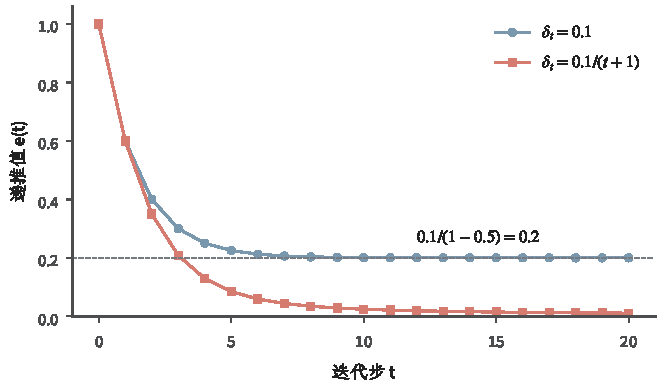
\includegraphics[width=\linewidth]{figures/01-mathematical-preliminaries/01-mathematical-language-combinatorics-analysis-optimization/matplotlib/analysis-geometry/language-perturbed-recurrence.pdf}
 \caption{相同初值与收缩系数下的两种递推。蓝线使用持续扰动，红线使用衰减扰动；每个点都是整数步上的精确递推值，图中$e(t)$对应正文的$e^{(t)}$，灰虚线是持续扰动留下的极限$0.2$。图为教学构造。}
 \label{fig:prelim-perturbed-recurrence}
\end{figure}

衰减扰动的结论可以直接由有限展开式~\eqref{eq:analysis-perturbed-distance-unrolling}核对。
给定$\varepsilon>0$，先选$S$使$s\geq S$时$\delta_s\leq\varepsilon(1-\rho)/2$。
对$t>S$把累计和拆成两段：前$S$项是有限个旧扰动，其权重随$t$几何趋零；后面的项满足
\[
 \sum_{s=S}^{t-1}\rho^{t-1-s}\delta_s
 \leq\frac{\varepsilon(1-\rho)}2\sum_{j=0}^{t-1-S}\rho^j
 \leq\frac\varepsilon2.
\]
旧扰动项和初始误差在充分大的$t$后也不超过$\varepsilon/2$，因此总误差趋于零。
这里需要$0\leq\rho<1$、$\delta_s\to0$和有限的初始误差；只写“每步误差很小”仍不足够。

\section{函数的连续性与局部变化}
\label{sec:analysis-local-models}

序列极限说明一族输入能否稳定；给定映射以后，还要判断这种稳定能否传到输出。
本节固定一个函数，分别考察输入扰动的控制、局部变化的计算及其近似误差。
由方程间接确定的函数需要额外证明解分支存在；经典可微性失效的函数则需要重新选择
变化信息。这些问题都针对函数本身，不要求先定义它的积分。

\subsection{连续性与扰动控制}
\label{sec:analysis-metric-continuity-extrema}

确定输入与输出的距离后，可以要求小的输入扰动只引起小的输出扰动。这就把熟悉的
实函数连续性推广到一般度量空间。
\Needspace{12\baselineskip}
\begin{definition}[度量空间中的连续映射]
\label{def:analysis-continuity}
设$(X,d_X)$与$(Y,d_Y)$为度量空间。函数$f:X\to Y$在$x\in X$处
\term{连续}（continuous），是指
\[
  \begin{gathered}
    \forall\varepsilon>0,\quad \exists\delta>0,\quad \forall x'\in X,\\
    d_X(x,x')<\delta\Longrightarrow d_Y\bigl(f(x),f(x')\bigr)<\varepsilon.
  \end{gathered}
\]
若$f$在每个$x\in X$处连续，则称$f$在$X$上连续。
\end{definition}
这里$\delta$可以依赖$x$和$\varepsilon$。等价地，只要$x_n\to x$，就有$f(x_n)\to f(x)$。连续函数因而允许把一个已经存在的极限送入函数：$f(\lim_n x_n)=\lim_n f(x_n)$。这里必须同时说明输入和输出采用的度量。

例如恒等映射$F(x)=x$从$(\mathbb R,d_1)$映到$(\mathbb R,d_2)$时处处不连续。
在任意$x$附近，总能找到通常距离任意小但不等于$x$的$x'$，它们的输出距离却始终为
$1$，无法小于$\varepsilon=1/2$。反过来，从$(\mathbb R,d_2)$到
$(\mathbb R,d_1)$的同一公式连续：选$\delta=1/2$，输入距离小于$\delta$就只可能
有$x'=x$，输出距离于是为$0$。这不是函数公式发生变化，而是输入输出空间对
“附近”的判断不同。图~\ref{fig:analysis-metric-convergence}右侧显示前一种失败。

\begin{figure*}[htbp]
  \centering
  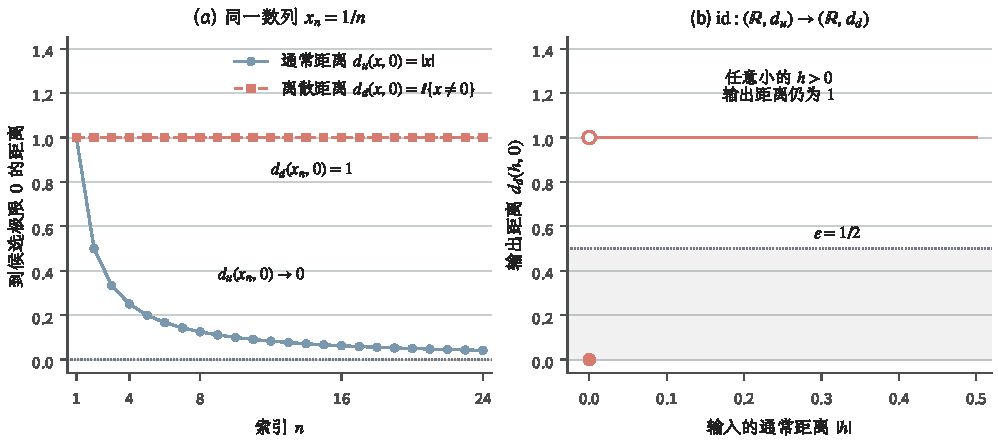
\includegraphics[width=\linewidth]{figures/01-mathematical-preliminaries/01-mathematical-language-combinatorics-analysis-optimization/matplotlib/analysis-concepts/analysis-metric-convergence.pdf}
  \caption{数值相同，距离不同。图中$d_u,d_d$分别对应正文的通常距离$d_1$与离散距离$d_2$。（a）数列 $x_n=1/n$ 到 $0$ 的通常距离趋于零，离散距离却恒为 $1$，所以收敛要连同度量说明。（b）恒等映射从通常度量空间映入离散度量空间时，任意非零且很小的输入位移仍对应输出距离 $1$，不能进入 $\varepsilon=1/2$ 的输出邻域，故它在 $0$ 处不连续。图为解析教学示例。}
  \label{fig:analysis-metric-convergence}
\end{figure*}

\begin{definition}[一致连续映射]
\label{def:analysis-uniform-continuity}
设$(X,d_X)$与$(Y,d_Y)$为度量空间，$f:X\to Y$。若对每个$\varepsilon>0$都能找到一个与具体位置无关的$\delta>0$，使任意
$x,x'\in X$只要$d_X(x,x')<\delta$便有
$d_Y(f(x),f(x'))<\varepsilon$，就称$f$\term{一致连续}
（uniformly continuous）。
\end{definition}
连续性允许不同位置使用不同的$\delta$，一致连续则要求同一个
$\delta$同时控制整个定义域。连续性本身并不足以给出这种统一控制：
$f(x)=x^2$在$\mathbb{R}$上连续，令$x\to+\infty$并取$x'=x+1/x$，可见输入距离趋于零而输出距离
$|f(x')-f(x)|=2+1/x^2$不趋于零。

\begin{definition}[Lipschitz连续映射]
\label{def:analysis-lipschitz-continuity}
设$(X,d_X)$与$(Y,d_Y)$为度量空间，$f:X\to Y$。若存在有限常数$L\geq0$，使所有$x,x'\in X$都满足
\begin{equation}
  d_Y\bigl(f(x),f(x')\bigr)\leq Ld_X(x,x'),
\label{eq:analysis-lipschitz-condition}
\end{equation}
则称$f$为$L$-\term{Lipschitz连续}（Lipschitz continuous）。
\end{definition}
它不仅用同一个
$\delta$控制整个定义域，还给出输出变化相对于输入变化的线性上界，因而蕴含一致连续。
函数$f(x)=\sqrt{x}$在$[0,1]$上满足$|\sqrt{x}-\sqrt{x'}|\leq\sqrt{|x-x'|}$，
因而选$\delta=\varepsilon^2$就得到一致连续性，却不能得到Lipschitz连续性：若存在有限$L$，
令$x'=0$便会要求$\sqrt{x}\leq Lx$，即$1/\sqrt{x}\leq L$，这在$x\downarrow0$时不可能成立。
同一个公式在不同定义域上可能具有不同的统一控制。$f(x)=x^2$在$[0,1]$上满足
$|x^2-z^2|\leq2|x-z|$，因而$2$-Lipschitz；在整个实线上却没有有限的全局Lipschitz
常数。这两个例子说明，统一的$\varepsilon$--$\delta$控制与线性误差上界仍是不同要求。

\term{局部Lipschitz函数}（locally Lipschitz function）要求每个点附近的函数变化
都能由某个有限Lipschitz常数控制。与全局Lipschitz条件不同，各个邻域可以使用不同的常数。
\begin{definition}[局部Lipschitz函数]
\label{def:analysis-local-lipschitz}
设$U\subseteq\mathbb{R}^d$为开集，$f:U\to\mathbb{R}$。若对每个$\bm{x}\in U$，
都存在半径$r>0$与有限常数$L\geq0$，使$B(\bm{x},r)\subseteq U$，并且
\[
  |f(\bm{y})-f(\bm{z})|
  \leq L\lVert\bm{y}-\bm{z}\rVert_2
  \quad\text{对所有 }\bm{y},\bm{z}\in B(\bm{x},r)\text{成立},
\]
则称$f$在$U$上局部Lipschitz。
\end{definition}

这里$r$与$L$可以依赖中心点；一旦邻域确定，同一个$L$须控制其中的任意两点。
例如$f(x)=x^2$在任意$(x_0-r,x_0+r)$上可取$L=2(|x_0|+r)$，所以在实轴上
局部Lipschitz，却不是全局Lipschitz。向量值函数也用输出范数替换绝对值，
作完全相同的局部定义。局部控制要提升为区域内的统一控制，还需要区域或导数的额外条件。


第~\ref{chap:sets-functions-and-proofs}章已区分下确界与最小值：数值可以逼近一个下界，却始终找不到达到它的点。
要让近似最优点最终提供一个可行解，需要防止点列逃向无穷远或被排除的边界。
在一般度量空间中，承担这一职责的是紧致性。
\begin{definition}[开覆盖与紧致性]
\label{def:analysis-compactness}
设$(X,d)$为度量空间，$K\subseteq X$。若一族$X$中的开集的并包含$K$，就称这族开集为$K$的
\term{开覆盖}（open cover）；若从中选出的有限个开集仍覆盖$K$，它们就构成
\term{有限子覆盖}（finite subcover）。集合$K$的每个开覆盖都能选出有限子覆盖时，
称$K$为\term{紧致}（compact）。
\end{definition}
在度量空间中，这一定义等价于
\term{序列紧致性}：集合中的每个序列都有一个子序列收敛到仍在该集合中的点。
后一种表述更适合分析算法产生的点列，因为它直接提供候选极限。

紧致性还能把逐点连续提升为一致连续：连续映射在紧致定义域上一定一致连续。
这为前面闭区间上的统一控制提供了一个一般条件，但不保证Lipschitz连续；
$\sqrt{x}$的例子已说明，输出变化未必能由输入距离的一次常数倍控制。

在有限维欧氏空间$\mathbb{R}^d$中，Heine--Borel定理说明紧致等价于闭且有界。这个结论不能原样搬到一般度量空间。考虑所有有界实数序列组成的空间
\[   \ell^\infty   =   \left\{\bm{x}=(x_1,x_2,\ldots):   \sup_{k\geq1}|x_k|<\infty\right\},   \qquad   d(\bm{x},\bm{y})=\sup_{k\geq1}|x_k-y_k|. \]
令$\bm{e}_n$只有第$n$个坐标为$1$，其余坐标为$0$。集合 $\{\bm{e}_n:n\geq1\}$有界，而且在$\ell^\infty$中是闭集；但$n\neq m$时 $d(\bm{e}_n,\bm{e}_m)=1$，所以任何子序列都不是柯西数列，更不可能收敛。一般空间中 “闭且有界”不足以替代紧致，正是因为无穷多个彼此分离的方向可能留在同一个有界球内。
\begin{theorem}[紧致集上的极值定理]
\label{thm:analysis-extreme-value}
设$K$是非空紧致度量空间，$f:K\to\mathbb{R}$连续，则$f$在$K$上同时达到最小值与最大值。
\end{theorem}
这里回顾熟悉的极值定理，不再展开证明。紧致性的两项作用是从近似最优点列中抽出收敛子序列，并保证极限仍在可行集合内。连续性随后把函数值极限传到该点。任一条件缺失都可能使最优解不存在。
\begin{example}[极值存在条件怎样失效]
\label{ex:analysis-extrema-failures}
在开区间$(0,1)$上，连续函数$f(x)=x$的下确界为$0$，却没有最小点；定义域不紧致， 极限点$0$被排除。把定义域改成闭但不紧致的$\mathbb{R}$，连续函数$f(x)=e^x$仍有下确界$0$而不达到它。另一方面，在紧致集合$[0,1]$上定义
\[   g(0)=1,\qquad g(x)=x\quad(x>0), \]
则$\inf g=0$也未达到；这次失败的是$g$在$0$处不连续。三个例子分别表明“连续”、 “闭”或“有界”中的单独一项都不是一般的极值存在保证。
\end{example}

连续性与可导性也应分开。回顾一元情形，导数要求左右两侧的差商趋向同一斜率，
比函数值趋近本身更强：$x^2$光滑，$|x|$在$0$连续但有尖点，
阈值函数$\mathbb I\{x\geq0\}$则在$0$跳跃。
尖点只阻止共同斜率，跳跃连共同的函数值极限也破坏了。
图~\ref{fig:analysis-continuity-counterexamples}把三者放在同一位置比较；
下一小节将写出差商和整体线性近似的正式条件。

\begin{figure*}[htbp]
  \centering
  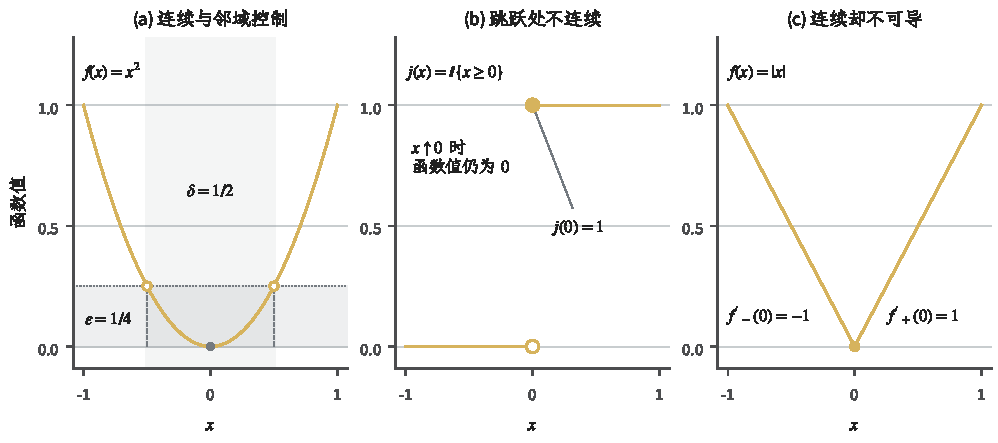
\includegraphics[width=\linewidth]{figures/01-mathematical-preliminaries/01-mathematical-language-combinatorics-analysis-optimization/matplotlib/analysis-concepts/analysis-continuity-counterexamples.pdf}
  \caption{三个不同的局部性质。（a）$f(x)=x^2$ 在 $0$ 处可用 $\delta=1/2$ 控制 $\varepsilon=1/4$：严格位于输入邻域内的点，其函数值严格落在输出邻域内。（b）阶跃函数在 $0$ 的左极限为 $0$，取值却为 $1$，空心点和实心点区分两者。（c）$|x|$ 在 $0$ 处连续，但左右导数分别为 $-1$ 和 $1$，不存在共同的双侧导数。图中曲线均为解析教学示例。}
  \label{fig:analysis-continuity-counterexamples}
\end{figure*}

\subsection{一阶导数与线性近似}
\label{sec:analysis-vector-chain-matrix-calculus}
\label{sec:analysis-derivatives-linear-approximation}
连续性只保证小扰动不会引起固定幅度的跳变；若还要预测变化的方向和大小，
就要寻找一个作用于扰动的线性映射。本节先建立这个近似，再处理不同输入输出形状：向量输出
需要Jacobian矩阵，复合映射需要串联两层线性变化，矩阵变量则需要用迹内积表示同一个
一阶变化。这里的“一阶”指对输入扰动保留线性项，与下一节研究斜率变化的二阶导数相对。

\subsubsection{导数与全微分}

从一元函数开始，把输出增量除以输入增量，得到这一小段上的平均变化率；
输入增量趋零后若仍有稳定值，就用它预测附近的输出。

一元函数$f:\mathbb{R}\to\mathbb{R}$在$x$处的\term{导数}（derivative）定义为
\[   f'(x)=\lim_{h\to0}\frac{f(x+h)-f(x)}{h}, \]
前提是这个双侧极限存在。它说明输入发生小变化$h$时，函数增量的一阶部分是$f'(x)h$：
\begin{equation}
  f(x+h)=f(x)+f'(x)h+o(|h|).
\label{eq:analysis-scalar-first-order}
\end{equation}
第~\ref{sec:comb-growth-scales}节的小$o$仍表示相对余项趋零，不过这里的趋向是$h\to0$：余项$r(h)$满足$r(h)/|h|\to0$，不只是$h$本身很小。导数存在必然推出函数在该点连续，但连续不保证可导，例如$|x|$在$0$处连续，左右导数却分别为 $-1$和$1$。
这也解释了图中尖点与跳跃的区别；两者都不能使用经典双侧导数，失效的层次却不同。

对$f:\mathbb{R}^d\to\mathbb{R}$，沿方向$\bm{v}\in\mathbb{R}^d$的
\term{方向导数}（directional derivative）是
\[   D_{\bm{v}}f(\bm{x})   =   \lim_{t\to0}   \frac{f(\bm{x}+t\bm{v})-f(\bm{x})}{t}. \]
取$\bm{v}$为第$j$个坐标方向$\bm{e}_j$，就得到\term{偏导数}
（partial derivative）$\partial f/\partial x_j$。方向导数只检查一条直线，而整体可微性要求所有小扰动共享同一个线性近似。

函数$f:\mathbb{R}^d\to\mathbb{R}$在$\bm{x}$处\term{可微}
（differentiable），是指存在一个线性映射 $A:\mathbb{R}^d\to\mathbb{R}$，使
\begin{equation}
  f(\bm{x}+\bm{h})
  =
  f(\bm{x})+A(\bm{h})+o(\lVert\bm{h}\rVert_2).
\label{eq:analysis-total-differentiability}
\end{equation}
线性部分$A(\bm h)$称为全微分，也记为$\mathrm df_{\bm x}(\bm h)$。
条件要求对任意趋零的非零扰动$\bm h$都有
$|f(\bm x+\bm h)-f(\bm x)-A(\bm h)|/\lVert\bm h\rVert_2\to0$，
而不是先固定一个方向，再允许误差控制随方向改变。
在欧氏空间中，每个这样的线性泛函都可写为 $A(\bm{h})=\langle\nabla f(\bm{x}),\bm{h}\rangle$，其中
\[   \nabla f(\bm{x})   =   \left(     \frac{\partial f}{\partial x_1}(\bm{x}),\ldots,     \frac{\partial f}{\partial x_d}(\bm{x})   \right)^{\top} \]
称为\term{梯度}（gradient）。因此梯度不是若干偏导数的随意排列，而是表示局部线性映射的向量；扰动$\bm{h}$通过内积变成函数的一阶变化。

可微必然推出所有方向导数存在，并且 $D_{\bm{v}}f(\bm{x})=\langle\nabla f(\bm{x}),\bm{v}\rangle$。反向结论不成立， 仅有偏导数更不够。
\begin{example}[偏导数存在但不可微]
\label{ex:analysis-partials-not-differentiable}
定义$f:\mathbb{R}^2\to\mathbb{R}$为
\[   f(x,y)=
\begin{cases}     \dfrac{xy}{\sqrt{x^2+y^2}}, & (x,y)\neq(0,0),\\[6pt]     0, & (x,y)=(0,0).
\end{cases} \]
沿两条坐标轴，函数恒为$0$，所以 $\partial f/\partial x(0,0)=\partial f/\partial y(0,0)=0$。若$f$在原点可微， 候选线性部分只能是零映射。可是沿$\bm{h}=(t,t)$，
\[   \frac{|f(t,t)-f(0,0)|}{\lVert(t,t)\rVert_2}   =   \frac{|t|/\sqrt{2}}{\sqrt{2}|t|}   =\frac12, \]
余项与$\lVert\bm{h}\rVert_2$之比不趋于零，故$f$在原点不可微。偏导数只看坐标轴，遗漏了其他接近路径。本例沿每个方向$\bm v=(a,b)$的
正向方向导数都存在，这里只令$t\downarrow0$，得到$ab/\sqrt{a^2+b^2}$（零方向取$0$）；它却不是关于$\bm v$
的线性函数，而且双侧方向导数在$ab\neq0$时不存在。方向极限采用单侧还是双侧，
必须与所用定义一致；本节定义采用双侧极限。
\end{example}

一个常用的充分条件是：若$f$的所有一阶偏导数在$\bm{x}$的某个邻域内存在，并在 $\bm{x}$处连续，则$f$在$\bm{x}$处可微。注意这只是方便核对的充分条件，不是必要条件； 可微函数的偏导数不一定在该点附近连续。

即使每个双侧方向导数都存在，也未必可微。例如令
$g(x,y)=x^3/(x^2+y^2)$于非零点，$g(0,0)=0$。
沿$\bm v=(a,b)\neq\bm0$有$D_{\bm v}g(0,0)=a^3/(a^2+b^2)$，
但坐标方向导数给出的候选梯度为$(1,0)^\top$，它对方向$(1,1)^\top$
预测$1$而非实际的$1/2$。这些方向变化率无法拼成一个线性映射。
与前例的单侧方向极限相比，这里直接检验了本节采用的双侧定义。

用$f(x)=x^3-3x$保留一个贯穿例子。在$x_0=1/2$处，
\[
  f(x_0)=-\frac{11}{8},\qquad f'(x_0)=3x_0^2-3=-\frac94.
\]
输入改变$h$时，一阶近似给出
\begin{equation}
  T_1(h)=f(x_0)+f'(x_0)h=-\frac{11}{8}-\frac94h.
\label{eq:analysis-cubic-linear-model}
\end{equation}
取$h=0.1$，$T_1(h)=-1.600$，而实际$f(0.6)=-1.584$。近似抓住了下降方向和主要
变化量，但还有$0.016$的误差；第~\ref{sec:analysis-second-order-curvature}节将用曲率解释这部分差别。
\subsubsection{复合映射与链式法则}

当一个输入产生多个输出时，每个输出都有一行局部线性系数，把这些行排在一起便得到
Jacobian矩阵。复合计算只需再把前一层的输出扰动作为后一层的输入扰动。
设$f:\mathbb{R}^d\to\mathbb{R}^m$。若存在矩阵 $\bm{J}_f(\bm{x})\in\mathbb{R}^{m\times d}$使
\begin{equation}
  f(\bm{x}+\bm{h})
  =
  f(\bm{x})+\bm{J}_f(\bm{x})\bm{h}
  +o(\lVert\bm{h}\rVert_2),
\label{eq:analysis-jacobian-linearization}
\end{equation}
则称$f$在$\bm{x}$处可微，$\bm{J}_f(\bm{x})$称为
\term{Jacobian矩阵}（Jacobian matrix）。其第$i,j$个元素是 $\partial f_i/\partial x_j$。矩阵有$m$行、$d$列，因为它把$d$维输入扰动映射成 $m$维输出扰动。

若$f$在$\bm{x}$处可微，且$g:\mathbb{R}^m\to\mathbb{R}^p$在$f(\bm{x})$处可微，则复合映射满足
\begin{equation}
  \bm{J}_{g\circ f}(\bm{x})
  =
  \bm{J}_g\bigl(f(\bm{x})\bigr)\bm{J}_f(\bm{x}).
\label{eq:analysis-vector-chain-rule}
\end{equation}
这就是\term{链式法则}（chain rule）。维度同时给出乘法次序： $(p\times m)(m\times d)=p\times d$，反向相乘往往没有定义。即使两个方阵能够交换书写顺序，矩阵乘法通常也不交换，不能据标量求导经验调换因子。

上面的$g$允许向量输出。当$p=1$时，$g$把中间向量变成一个标量。在优化问题中，
这个标量通常是待最小化的目标值，本书便把此时的$g$记为$\ell$。令
$\bm y=f(\bm x)$，总目标就是$L(\bm x)=\ell(f(\bm x))$；$\ell$只是原复合映射的
最后一层，并没有增加一个未说明的输出。采用列向量梯度，链式法则写成
\[
  \nabla L(\bm x)
  =\bm J_f(\bm x)^\top\nabla\ell(\bm y)\big|_{\bm y=f(\bm x)}.
\]
局部线性映射在前向计算中按$\bm J_f$作用，在标量目标的反向计算中按转置
$\bm J_f^\top$传回。这是后续反向传播的线性代数核心，具体网络结构留到模型章节。

\begin{example}[从中间向量求回复合目标的梯度]
\label{ex:analysis-chain-rule-calculation}
令
\[
  f(x_1,x_2)=(x_1^2,x_1x_2,x_2)^\top,
  \qquad \ell(\bm y)=\frac12(y_1^2+y_2^2+y_3^2).
\]
$f$从二维输入产生三维中间量，$\ell$再把三维中间量变成一个数。于是
\[
  \bm J_f=\begin{bmatrix}2x_1&0\\x_2&x_1\\0&1\end{bmatrix},
  \qquad \nabla\ell(\bm y)=\bm y.
\]
在$\bm x=(1,2)^\top$处，$\bm y=(1,2,2)^\top$，链式法则给出
\[
  \nabla L(1,2)
  =\begin{bmatrix}2&2&0\\0&1&1\end{bmatrix}
    \begin{bmatrix}1\\2\\2\end{bmatrix}
  =\begin{bmatrix}6\\4\end{bmatrix}.
\]
也可以把复合函数直接展开为
$L(x_1,x_2)=\tfrac12(x_1^4+x_1^2x_2^2+x_2^2)$，求偏导得到
$\nabla L=(2x_1^3+x_1x_2^2,\,x_1^2x_2+x_2)^\top$，在同一点仍为$(6,4)^\top$。
两种计算处理同一个目标；链式形式保留了中间映射，可分别复用各层的导数。
矩阵形状$(2\times3)(3\times1)=2\times1$也核对了梯度传递的次序。
\end{example}

若要把任意实数评分变成正数且总和为$1$的权重，可以先取指数再除以共同的总和。
这就是$n$维\term{归一化指数映射}（softmax）。对
$\bm{z}\in\mathbb{R}^n$，令
\[
  s_i(\bm{z})
  =
  \frac{e^{z_i}}{\sum_{k=1}^n e^{z_k}},
  \qquad i=1,\ldots,n.
\]
记分母为$Z=\sum_k e^{z_k}$。指数函数求导和商法则给出
\[
  \frac{\partial s_i}{\partial z_j}
  =
  \frac{\mathbb{I}\{i=j\}e^{z_i}Z-e^{z_i}e^{z_j}}{Z^2}
  =
  s_i\bigl(\mathbb{I}\{i=j\}-s_j\bigr).
\]
因此整个Jacobian矩阵为
\begin{equation}
  \bm{J}_{\bm{s}}(\bm{z})
  =
  \operatorname{diag}(\bm{s})-\bm{s}\bm{s}^{\top}.
\label{eq:analysis-softmax-jacobian}
\end{equation}
对角项$s_i(1-s_i)$描述提高$z_i$对自身分量的影响，非对角项$-s_is_j$
来自共同分母：提高一个坐标会压低其余归一化分量。每行元素之和为零，
这也与给所有$z_i$同时加同一常数不改变输出相符。
\subsubsection{矩阵变量与微分计算}

如果输入本身是矩阵，逐条写出$mn$个偏导数会掩盖原有的矩阵乘法结构。矩阵$\bm{X}\in\mathbb{R}^{m\times n}$可以看成$mn$个坐标组成的对象，矩阵梯度则把这些一阶变化重新排回原来的形状。先固定Frobenius迹内积
\[   \langle\bm{A},\bm{B}\rangle_F   =   \operatorname{tr}(\bm{A}^{\top}\bm{B}) \]
其中$\operatorname{tr}$是方阵对角元素之和，所以这个内积也等于
$\sum_{i,j}\bm A_{i,j}\bm B_{i,j}$，对应范数为
$\lVert\bm H\rVert_F=(\sum_{i,j}\bm H_{i,j}^2)^{1/2}$。
对标量函数$f(\bm X)$，全微分要求
$f(\bm X+\bm H)=f(\bm X)+\mathrm df_{\bm X}(\bm H)+o(\lVert\bm H\rVert_F)$。
用这个内积
定义矩阵梯度：若一阶全微分能够写成
\begin{equation}
  \mathrm{d}f
  =
  \langle\nabla_{\bm{X}}f,\mathrm{d}\bm{X}\rangle_F
  =
  \operatorname{tr}\bigl((\nabla_{\bm{X}}f)^{\top}
  \mathrm{d}\bm{X}\bigr),
\label{eq:analysis-matrix-gradient-definition}
\end{equation}
则$\nabla_{\bm{X}}f$与$\bm{X}$形状相同。计算时可先用乘积法则展开微分，再利用
\[   \operatorname{tr}(\bm{A}\bm{B})   =\operatorname{tr}(\bm{B}\bm{A}),\qquad   \operatorname{tr}(\bm{A}\bm{B}\bm{C})   =\operatorname{tr}(\bm{B}\bm{C}\bm{A}), \]
把$\mathrm{d}\bm{X}$移动到末端。迹只允许循环移位，不能任意交换相邻矩阵。

先考虑二次型$q(\bm{x})=\bm{x}^{\top}\bm{A}\bm{x}$，其中 $\bm{A}\in\mathbb{R}^{d\times d}$固定。由乘积法则，
\begin{align*}
  \mathrm{d}q
  &=
  (\mathrm{d}\bm{x})^{\top}\bm{A}\bm{x}
  +\bm{x}^{\top}\bm{A}\,\mathrm{d}\bm{x}\\
  &=
  \bm{x}^{\top}(\bm{A}^{\top}+\bm{A})\,\mathrm{d}\bm{x}.
\end{align*}
因此
\begin{equation}
  \nabla_{\bm{x}}
  \bigl(\bm{x}^{\top}\bm{A}\bm{x}\bigr)
  =
  (\bm{A}+\bm{A}^{\top})\bm{x}.
\label{eq:analysis-quadratic-form-gradient}
\end{equation}
只有当$\bm{A}$对称时才能化为$2\bm{A}\bm{x}$。直接写成$2\bm{A}\bm{x}$会悄然加入对称性条件。

对固定的$\bm{A}\in\mathbb{R}^{m\times n}$，令 $f(\bm{X})=\operatorname{tr}(\bm{A}^{\top}\bm{X})$。它的微分已经符合式
\eqref{eq:analysis-matrix-gradient-definition}，所以
\begin{equation}
  \nabla_{\bm{X}}\operatorname{tr}(\bm{A}^{\top}\bm{X})
  =\bm{A}.
\label{eq:analysis-trace-linear-gradient}
\end{equation}
这个简单关系常用于从迹表达式中读出梯度。

若方阵$\bm{X}$可逆，由恒等式$\bm{X}\bm{X}^{-1}=\bm{I}$取微分可得
\[   (\mathrm{d}\bm{X})\bm{X}^{-1}   +\bm{X}\,\mathrm{d}(\bm{X}^{-1})=\bm{0}. \]
左乘$\bm{X}^{-1}$后得到
\begin{equation}
  \mathrm{d}(\bm{X}^{-1})
  =
  -\bm{X}^{-1}(\mathrm{d}\bm{X})\bm{X}^{-1}.
\label{eq:analysis-inverse-differential}
\end{equation}
两个$\bm{X}^{-1}$位于扰动两侧，不能合并成 $-\bm{X}^{-2}\mathrm{d}\bm{X}$，因为$\mathrm{d}\bm{X}$未必与$\bm{X}^{-1}$交换。

最后设$\bm{X}\in\mathbb{R}^{d\times d}$正定，因而$\det\bm{X}>0$且 $\log\det\bm{X}$有定义。Jacobi行列式公式给出
\[   \mathrm{d}\det\bm{X}   =   \det(\bm{X})\operatorname{tr}   (\bm{X}^{-1}\mathrm{d}\bm{X}). \]
再应用标量对数的链式法则，
\begin{equation}
  \mathrm{d}\log\det\bm{X}
  =
  \operatorname{tr}(\bm{X}^{-1}\mathrm{d}\bm{X}),
  \qquad
  \nabla_{\bm{X}}\log\det\bm{X}
  =
  \bm{X}^{-\top}.
\label{eq:analysis-logdet-gradient}
\end{equation}
正定矩阵对称，所以$\bm{X}^{-\top}=\bm{X}^{-1}$；对一般可逆实矩阵， $\log\det\bm{X}$还需要$\det\bm{X}>0$，而梯度应保留转置。以上推导依赖的不是元素级记忆口诀，而是局部线性近似、乘积次序和迹内积三件事。
\begin{example}[逆矩阵微分中的乘法次序]
\label{ex:analysis-noncommuting-inverse-differential}
取$\bm X=\operatorname{diag}(2,1)$，扰动方向
$\bm E=\begin{bmatrix}0&1\\1&0\end{bmatrix}$。沿$\bm X+t\bm E$求逆矩阵的导数为
\[
 -\bm X^{-1}\bm E\bm X^{-1}
 =\begin{bmatrix}0&-1/2\\-1/2&0\end{bmatrix}.
\]
若照搬标量规则而写成$-\bm X^{-2}\bm E$，会得到
$\begin{bmatrix}0&-1/4\\-1&0\end{bmatrix}$，连对称性都丢失。
原路径在$0$附近由对称可逆矩阵组成，其逆与导数也应对称；这一结构检查能直接发现错误。
矩阵变量沿给定方向微分时，夹在两侧的逆矩阵不能随意移到同一侧。
\end{example}

\subsubsection{导数界与位移控制}

一点处的线性近似还不能控制一段有限位移。若沿整段路径的变化率都有上界，
中值定理才能把局部信息变成端点之间的误差界。
若$a<b$，$f:[a,b]\to\mathbb{R}$在$[a,b]$上连续、在$(a,b)$上可导，则
\term{中值定理}（mean value theorem）保证存在$c\in(a,b)$使
\begin{equation}
  f(b)-f(a)=f'(c)(b-a).
\label{eq:analysis-mean-value-theorem}
\end{equation}
所以，若区间上$|f'(x)|\leq L$，便有$|f(b)-f(a)|\leq L|b-a|$。这说明有界导数可以推出Lipschitz控制。多元标量函数也可沿线段使用一元中值定理：当连接 $\bm{x}$与$\bm{y}$的线段位于定义域且$f$在线段邻域可微时，
\[   |f(\bm{y})-f(\bm{x})|   \leq   \sup_{0\leq t\leq1}   \lVert\nabla f(\bm{x}+t(\bm{y}-\bm{x}))\rVert_2   \lVert\bm{y}-\bm{x}\rVert_2. \]
这里控制的是标量函数值差。对向量值函数，不能一般地断言存在一个共同的$c$让整个向量增量等于单个Jacobian矩阵乘以输入增量；应使用积分形式或范数上界。

对向量输出，用线性映射的最大放大倍数替代标量导数的绝对值。
\begin{definition}[欧氏诱导算子范数]
\label{def:analysis-induced-operator-norm}
对矩阵
$\bm{A}\in\mathbb{R}^{s\times r}$，由欧氏范数\term{诱导的算子范数}
（induced operator norm）定义为
\[
  \lVert\bm{A}\rVert_{\mathrm{op}}
  =
  \sup_{\bm{h}\neq\bm{0}}
  \frac{\lVert\bm{A}\bm{h}\rVert_2}{\lVert\bm{h}\rVert_2}
  =
  \sup_{\lVert\bm{h}\rVert_2=1}\lVert\bm{A}\bm{h}\rVert_2.
\]
\end{definition}
它表示线性映射对向量长度的最大放大倍数，定义立即给出
$\lVert\bm{A}\bm{h}\rVert_2
\leq\lVert\bm{A}\rVert_{\mathrm{op}}\lVert\bm{h}\rVert_2$。
例如$\bm A=\operatorname{diag}(2,1)$把第一坐标放大两倍、第二坐标保持不变，
故$\lVert\bm A\rVert_{\mathrm{op}}=2$；最大放大由第一坐标方向达到。
下文$\bm DG$与$\bm J_G$均表示$G$的Jacobian矩阵。
若映射$G$在包含$\bm{y}'$到$\bm{y}$线段的开邻域内连续可微，可以沿线段使用一元中值定理，得到
\begin{equation}
  \begin{aligned}
  \lVert G(\bm{y})-G(\bm{y}')\rVert_2
  &\leq
  \sup_{0\leq t\leq1}
  \left\lVert
    \bm{D}G\bigl(\bm{y}'+t(\bm{y}-\bm{y}')\bigr)
  \right\rVert_{\mathrm{op}}
  \lVert\bm{y}-\bm{y}'\rVert_2.
  \end{aligned}
\label{eq:analysis-operator-mean-value-bound}
\end{equation}
这个向量上界无需预先使用积分公式。若$\bm u=G(\bm y)-G(\bm y')\neq\bm0$，
取单位向量$\bm v=\bm u/\lVert\bm u\rVert_2$，并沿线段定义标量函数
$\phi(t)=\bm v^\top G(\bm y'+t(\bm y-\bm y'))$。
中值定理给出某个$\tau\in(0,1)$，使
\[
 \lVert\bm u\rVert_2
 =\phi(1)-\phi(0)
 =\bm v^\top\bm DG(\bm y'+\tau(\bm y-\bm y'))(\bm y-\bm y').
\]
对右侧使用欧氏内积与算子范数的上界便得到式~\eqref{eq:analysis-operator-mean-value-bound}；
$\bm u=\bm0$时该界直接成立。
因此，邻域内统一的导数范数上界会直接变成Lipschitz常数；若该上界小于$1$，就得到
第~\ref{sec:analysis-complete-contraction}节已经建立的压缩条件。

\subsection{二阶导数与局部曲率}
\label{sec:analysis-second-order-curvature}

延续$f(x)=x^3-3x$的例子，一阶导数$f'(x)=3x^2-3$还随位置变化。再求一次导数，
得到$f''(x)=6x$，所以$f''(1/2)=3$。在$x_0=1/2$附近，斜率向右移动时增大，
曲线向上弯；这解释了真实值为何高于前节的切线预测。图~\ref{fig:analysis-derivative-orders}将切线和下面的二次修正放在同一幅曲线图上比较。加入二次项得到
\begin{equation}
  T_2(h)=T_1(h)+\frac12f''(x_0)h^2
        =-\frac{11}{8}-\frac94h+\frac32h^2.
\label{eq:analysis-cubic-quadratic-model}
\end{equation}
在$h=0.1$时，$T_2=-1.585$，与实际值$-1.584$只差$0.001$。
一阶导数回答此处沿给定方向增还是减，二阶导数回答这个变化率怎样改变。
下一节再用Taylor展开给出一阶和二阶余项的完整表达式。

一阶近似只保留函数的局部斜率。若还要判断这个斜率怎样随位置改变，就需要
\term{Hessian矩阵}（Hessian matrix）。设$f:\mathbb{R}^d\to\mathbb{R}$在 $\bm{x}$附近二阶可微，定义
\[   \nabla^2 f(\bm{x})   =
\begin{bmatrix}     \dfrac{\partial^2 f}{\partial x_1^2} &     \cdots &     \dfrac{\partial^2 f}{\partial x_1\partial x_d}\\     \vdots & \ddots & \vdots\\     \dfrac{\partial^2 f}{\partial x_d\partial x_1} &     \cdots &     \dfrac{\partial^2 f}{\partial x_d^2}
\end{bmatrix}. \]
若二阶偏导数在邻域内连续，混合偏导数可以交换，Hessian矩阵因而对称。对方向 $\bm{v}$，二次型 $\bm{v}^{\top}\nabla^2f(\bm{x})\bm{v}$是沿直线 $t\mapsto f(\bm{x}+t\bm{v})$在$t=0$处的二阶导数。它衡量的不是函数值大小，而是沿该方向的一阶斜率变化。

对二次函数
\[   f(\bm{x})   =   \frac12\bm{x}^{\top}\bm{A}\bm{x}   +\bm{b}^{\top}\bm{x}+c, \]
只有$\bm{A}$的对称部分影响函数值。令 $\bm{H}=(\bm{A}+\bm{A}^{\top})/2$，则 $\nabla f(\bm{x})=\bm{H}\bm{x}+\bm{b}$且 $\nabla^2f(\bm{x})=\bm{H}$。正特征值对应向上弯曲的方向，负特征值对应向下弯曲的方向；特征值绝对值相差很大时，不同方向的尺度也相差很大。

\subsection{Taylor展开与余项控制}
\label{sec:analysis-taylor-approximation}
一阶导数给出切线，二阶导数描述斜率的变化，但近似不限于这两个阶数。Taylor展开
把函数在一点处的各阶导数组织成多项式，并用余项记录被舍弃的变化。
它承接前两节的导数计算，回答“保留多少信息能得到多准确的局部近似”，
而不把展开限定为二阶公式。

回顾一元Taylor公式：取非负整数$r$，若$f$在连接$x_0$与$x_0+h$的线段的开邻域上
$r+1$阶连续可微，且$h\neq0$，则存在两端之间的$\xi$使
\begin{equation}
  f(x_0+h)=\sum_{k=0}^{r}\frac{f^{(k)}(x_0)}{k!}h^k
  +\frac{f^{(r+1)}(\xi)}{(r+1)!}h^{r+1}.
\label{eq:analysis-taylor-arbitrary-order}
\end{equation}
约定$f^{(0)}=f$，$r$是所保留的最高次数。常数项记录当前函数值，线性项记录斜率，
二次项记录曲率，继续保留高阶项才得到更高阶近似。若沿这条线段
$|f^{(r+1)}|\leq M$，余项的绝对值便不超过$M|h|^{r+1}/(r+1)!$。
所以“高阶近似更准确”还依赖扰动尺度与导数上界，不能只比较多项式的次数。
此处给出的是选取某个中间点的Lagrange余项；若要保留整条线段上各位置的贡献，
第~\ref{sec:analysis-integration-remainders}节将由分部积分建立积分余项，
本节的极值判据并不依赖尚未建立的积分公式。

对前两节的$f(x)=x^3-3x$、$x_0=1/2$，三阶展开恰好为
\[
  f(x_0+h)=-\frac{11}{8}-\frac94h+\frac32h^2+h^3.
\]
此处所有四阶及以上导数为零，没有继续舍弃的项。一阶近似$T_1$与二阶近似$T_2$
分别舍弃$\tfrac32h^2+h^3$和$h^3$。图~\ref{fig:analysis-derivative-orders}把两侧扰动放在
同一尺度上比较，显示线性、二次近似怎样接近原曲线，并标出$h=\pm0.1$时的余项。

\begin{figure*}[htbp]
  \centering
  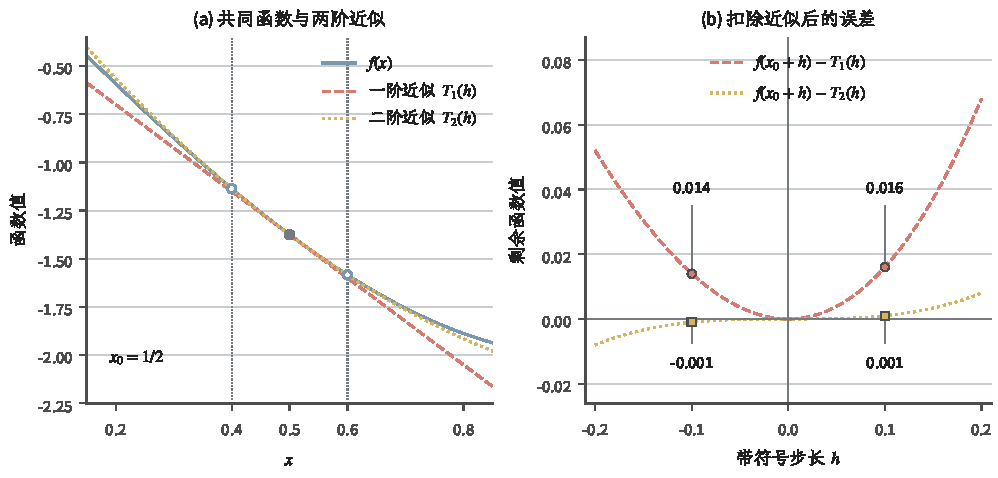
\includegraphics[width=\linewidth]{figures/01-mathematical-preliminaries/01-mathematical-language-combinatorics-analysis-optimization/matplotlib/analysis-concepts/analysis-derivative-orders.pdf}
  \caption{统一函数 $f(x)=x^3-3x$ 在 $x_0=1/2$ 处的两阶近似，记 $h=x-x_0$。（a）蓝线为真函数，红虚线为切线近似 $T_1=f(x_0)+f'(x_0)h$，黄点线加入二次项 $f''(x_0)h^2/2$，得到 $T_2$。（b）扣除各近似后的带符号余项分别为 $3h^2/2+h^3$ 与 $h^3$，标出 $h=\pm0.1$ 的精确结果。一阶导数确定切线，二阶导数补充局部曲率；余项的正负表示真值位于近似值的哪一侧。图为解析教学示例。}
  \label{fig:analysis-derivative-orders}
\end{figure*}


设连接$\bm{x}$与$\bm{x}+\bm{h}$的线段包含在一个开集内，并且$f$在该开集上二阶连续可微。对一元函数$\phi(t)=f(\bm{x}+t\bm{h})$使用Taylor定理，存在 $\theta\in(0,1)$使
\begin{equation}
  f(\bm{x}+\bm{h})
  =
  f(\bm{x})
  +\nabla f(\bm{x})^{\top}\bm{h}
  +\frac12
  \bm{h}^{\top}
  \nabla^2f(\bm{x}+\theta\bm{h})
  \bm{h}.
\label{eq:analysis-second-order-taylor}
\end{equation}
由Hessian矩阵的连续性，当$\bm{h}\to\bm{0}$时，中间点处的二阶项可以换成基点处的
二阶项，并把差异归入更小阶的余项：
\begin{equation}
  f(\bm{x}+\bm{h})
  =
  f(\bm{x})
  +\nabla f(\bm{x})^{\top}\bm{h}
  +\frac12\bm{h}^{\top}\nabla^2f(\bm{x})\bm{h}
  +o(\lVert\bm{h}\rVert_2^2).
\label{eq:analysis-second-order-local-model}
\end{equation}
式~\eqref{eq:analysis-second-order-local-model}是局部结论。若要在一个区域内给出统一余项界，还需控制该区域上的Hessian矩阵连续性或Lipschitz常数，不能仅凭一点处的二阶导数。


有了余项控制，才能由近似多项式判断函数本身的极值。局部极小点是指某个邻域内
所有函数值都不小于该点的值；严格局部极小还要求其他点的值严格更大。
设$\bm{x}^{\star}$是开集内部的局部极小点，且$f$在该点可微。对每个方向 $\bm{v}$考察$f(\bm{x}^{\star}+t\bm{v})$，一元函数的必要条件给出 $\nabla f(\bm{x}^{\star})^{\top}\bm{v}=0$。这对所有$\bm{v}$成立，因此
\begin{equation}
  \nabla f(\bm{x}^{\star})=\bm{0}.
\label{eq:analysis-first-order-necessary}
\end{equation}
若$f$还在该点二阶可微，同样沿任意方向使用一元二阶必要条件，可得
\begin{equation}
  \bm{v}^{\top}\nabla^2f(\bm{x}^{\star})\bm{v}\geq0
  \quad\text{对所有 }\bm{v},
\label{eq:analysis-second-order-necessary}
\end{equation}
即Hessian矩阵半正定。局部极大点对应半负定。这些只是必要条件：
$f(x)=x^4$与$f(x)=-x^4$在$0$处分别有严格局部极小值和严格局部极大值，
二者的二阶导数却都为零；$f(x)=x^3$在$0$处的一阶导数和二阶导数也都为零，
却没有极值。Hessian矩阵半正定或半负定本身不能决定驻点类型。

正定Hessian矩阵给出更强的充分条件。若$f$在$\bm{x}^{\star}$的某个邻域内二阶连续
可微，$\nabla f(\bm{x}^{\star})=\bm{0}$且
$\nabla^2f(\bm{x}^{\star})$正定，则其最小特征值为某个$\lambda>0$。由Hessian矩阵的
连续性，充分靠近$\bm{x}^{\star}$时，任意方向上的二次型仍至少为
$(\lambda/2)\lVert\bm{h}\rVert_2^2$。用式~\eqref{eq:analysis-second-order-taylor}
的中间点表达式，即可把这个曲率下界变成函数值下界；具体地，充分靠近时有
\[   f(\bm{x}^{\star}+\bm{h})-f(\bm{x}^{\star})   \geq   \frac{\lambda}{4}\lVert\bm{h}\rVert_2^2>0 \]
对充分小的非零$\bm{h}$成立，故$\bm{x}^{\star}$是严格局部极小点。负定情形给出严格局部极大点。

若驻点处Hessian矩阵既有正特征值又有负特征值，沿相应特征向量的小扰动会使函数值分别增加和减小，该点称为\term{鞍点}（saddle point）。例如 $f(x,y)=x^2-y^2$的原点就是鞍点。若Hessian矩阵仅半正定或含零特征值，二阶判据可能没有结论，必须查看更高阶项或函数的其他结构。上述必要条件还假定点位于无约束开集内部； 边界极小点的梯度可以不为零，受约束问题需要后续章节的可行方向与乘子条件。

\subsection{隐函数与解的敏感性}
\label{sec:analysis-implicit-parameter-integral}

链式法则计算已给定映射的变化；方程$F(\bm x,\bm y)=\bm0$却还没有直接给出
$\bm y$关于$\bm x$的函数。需要先证明局部解分支存在、唯一且可微，才能对它求导。
前面的导数位移界与本章压缩定理现在共同提供这一保证；驻点方程随后把解分支用于
参数变化下的敏感性分析。

显式关系$y=\varphi(x)$直接给出输入如何映射到输出，方程 $F(x,y)=0$却只规定二者必须共同满足的约束。例如 $F(x,y)=y^2-x=0$在$x>0$附近有$y=\sqrt{x}$和$y=-\sqrt{x}$两支，若不先指定所考察的解，方程并不定义唯一函数。更糟的是，在$(x,y)=(0,0)$附近，两支相交且 $\partial F/\partial y=2y=0$，不能把$y$稳定地看作$x$的可微函数。

\begin{theorem}[隐函数定理]
\label{thm:analysis-implicit-function}
设$F:\mathbb{R}^p\times\mathbb{R}^m\to\mathbb{R}^m$在 $(\bm{a},\bm{b})$的某个开邻域内连续可微， $F(\bm{a},\bm{b})=\bm{0}$，并且关于待解变量的Jacobian矩阵 \[   \bm{D}_{\bm{y}}F(\bm{a},\bm{b})   \in\mathbb{R}^{m\times m} \]
可逆。则存在$\bm{a}$与$\bm{b}$的邻域$U,V$，以及唯一的连续可微函数
$\varphi:U\to V$，使$\varphi(\bm{a})=\bm{b}$，并且对所有
$(\bm{x},\bm{y})\in U\times V$都有
\[
  F(\bm{x},\bm{y})=\bm{0}
  \quad\Longleftrightarrow\quad
  \bm{y}=\varphi(\bm{x}).
\]
其Jacobian矩阵满足
\begin{equation}
  \bm{D}\varphi(\bm{x})
  =
  -
  \bigl[\bm{D}_{\bm{y}}F(\bm{x},\varphi(\bm{x}))\bigr]^{-1}
  \bm{D}_{\bm{x}}F(\bm{x},\varphi(\bm{x})).
\label{eq:analysis-implicit-derivative}
\end{equation}
\end{theorem}

\begin{proof}
为证明定理~\ref{thm:analysis-implicit-function}的存在性，先把方程改写为局部压缩迭代。记
\[   \bm{A}   =   \bm{D}_{\bm{y}}F(\bm{a},\bm{b}),   \qquad   T_{\bm{x}}(\bm{y})   =   \bm{y}-\bm{A}^{-1}F(\bm{x},\bm{y}). \]
$F(\bm{x},\bm{y})=\bm{0}$当且仅当$\bm{y}$是$T_{\bm{x}}$的不动点。并且
\[   \bm{D}_{\bm{y}}T_{\bm{x}}(\bm{y})   =   \bm{I}   -   \bm{A}^{-1}\bm{D}_{\bm{y}}F(\bm{x},\bm{y}), \]
它在$(\bm{a},\bm{b})$处为零。由导数连续性，可以选择闭球 $B=\{\bm{y}:\lVert\bm{y}-\bm{b}\rVert_2\leq r\}$和$\bm{a}$的邻域$U$，使
\begin{equation}
  \sup_{\bm{x}\in U,\,\bm{y}\in B}
  \left\lVert
    \bm{D}_{\bm{y}}T_{\bm{x}}(\bm{y})
  \right\rVert_{\mathrm{op}}
  \leq q<1.
\label{eq:analysis-ift-uniform-contraction}
\end{equation}
沿$\bm{y}$方向使用式~\eqref{eq:analysis-operator-mean-value-bound}可知，每个
$T_{\bm{x}}$在$B$上都是同一因子$q$的压缩映射。

还必须核对自映射。因为$T_{\bm{a}}(\bm{b})=\bm{b}$且$T_{\bm{x}}(\bm{b})$关于 $\bm{x}$连续，可进一步缩小$U$，使
\[   \lVert T_{\bm{x}}(\bm{b})-\bm{b}\rVert_2   \leq\frac{1-q}{2}r. \]
于是对$\bm{y}\in B$，
\[
  \lVert T_{\bm{x}}(\bm{y})-\bm{b}\rVert_2
  \leq
  q\lVert\bm{y}-\bm{b}\rVert_2+\frac{1-q}{2}r
  \leq
  \frac{1+q}{2}r
  <r.
\]
所以$T_{\bm{x}}(B)$包含在$B$的内部$V$中。闭球$B$在有限维欧氏空间中完备，Banach
定理便对每个$\bm{x}\in U$给出唯一不动点$\varphi(\bm{x})\in V$。若
$(\bm{x},\bm{y})\in U\times V$且$F(\bm{x},\bm{y})=\bm{0}$，则$\bm{y}\in B$也是
$T_{\bm{x}}$的不动点，唯一性迫使$\bm{y}=\varphi(\bm{x})$。这证明了定理所述的局部
存在与零点集合的逐点唯一性。

还需说明所得解随参数连续可微。把$U$进一步缩小为开球，并使
$\overline U\times B$包含在原定义域内；这个集合紧致，关于$\bm x$的导数连续，
故有统一范数上界$L$。对$\bm x,\bm x'\in U$，
两点间的线段仍在$U$内，式~\eqref{eq:analysis-operator-mean-value-bound}
可用于$T_{\bm x}(\bm y)$的参数变化。利用两个不动点关系，
\[   \lVert\varphi(\bm{x})-\varphi(\bm{x}')\rVert_2   \leq   q\lVert\varphi(\bm{x})-\varphi(\bm{x}')\rVert_2   +L\lVert\bm{x}-\bm{x}'\rVert_2, \]
移项得到$\lVert\varphi(\bm x)-\varphi(\bm x')\rVert_2
\leq L\lVert\bm x-\bm x'\rVert_2/(1-q)$，
故$\varphi$局部Lipschitz连续。令 $\bm{h}\to\bm{0}$并记 $\bm{k}=\varphi(\bm{x}+\bm{h})-\varphi(\bm{x})$，前述界给出 $\lVert\bm{k}\rVert_2=O(\lVert\bm{h}\rVert_2)$。对恒等式
\[   F(\bm{x}+\bm{h},\varphi(\bm{x})+\bm{k})   -   F(\bm{x},\varphi(\bm{x}))   =   \bm{0} \]
作一阶展开，得到
\[   \bm{D}_{\bm{x}}F\,\bm{h}   +   \bm{D}_{\bm{y}}F\,\bm{k}   +   o(\lVert\bm{h}\rVert_2)   =   \bm{0}. \]
展开中的Jacobian均在$(\bm x,\varphi(\bm x))$处取值，联合扰动的余项
$o(\lVert(\bm h,\bm k)\rVert_2)$因$\lVert\bm k\rVert_2=O(\lVert\bm h\rVert_2)$
成为$o(\lVert\bm h\rVert_2)$。
基点的$\det\bm A\neq0$，行列式又是矩阵元素的连续函数，
所以邻域足够小时$\bm D_{\bm y}F$仍可逆。于是
\[   \bm{k}   =   -   (\bm{D}_{\bm{y}}F)^{-1}   \bm{D}_{\bm{x}}F\,\bm{h}   +   o(\lVert\bm{h}\rVert_2). \]
这证明$\varphi$可微并给出式~\eqref{eq:analysis-implicit-derivative}；各Jacobian矩阵连续又保证$\bm{D}\varphi$连续。至此，隐函数定理中的存在、局部唯一与导数公式都已得到说明。证明中特别核对了自映射和统一压缩条件，只有形式上的固定点改写并不足够。
\end{proof}

存在性、局部唯一性和可微性都需要证明，不能由形式求导代替。上面的证明已经核对这些条件。只看导数公式时，对恒等式 $F(\bm{x},\varphi(\bm{x}))=\bm{0}$应用链式法则，得到
\[   \bm{D}_{\bm{x}}F   +   \bm{D}_{\bm{y}}F\,\bm{D}\varphi   =   \bm{0}. \]
左乘$\bm{D}_{\bm{y}}F$的逆即得式~\eqref{eq:analysis-implicit-derivative}。乘法次序由矩阵维度决定，不能把逆矩阵随意移到右侧。


考虑依赖参数$\theta$的无约束目标$q(z,\theta)$。若局部最优解$z^\star(\theta)$位于定义域内部，它满足驻点方程
\[   F(\theta,z)   =   \frac{\partial q}{\partial z}(z,\theta)   =   0. \]
若$q$二阶连续可微，且 $\partial^2q/\partial z^2$在所考察解处非零，隐函数定理给出该驻点的局部唯一分支。这并不自动说明它是全局最优解；还要由曲率或其他结构核对最优性。
\begin{example}[参数二次目标中的解导数与包络导数]
\label{ex:analysis-parametric-quadratic}
对$\theta>-1$，令
\[   q(z,\theta)   =   \frac12(1+\theta)z^2-\theta z. \]
因为$\theta>-1$，配方得到
\[
  q(z,\theta)=\frac{1+\theta}{2}
  \left(z-\frac{\theta}{1+\theta}\right)^2
  -\frac{\theta^2}{2(1+\theta)}.
\]
平方项的系数为正，所以唯一驻点就是全局最小点。驻点方程为
\[   F(\theta,z)=(1+\theta)z-\theta=0. \]
隐式求导给出
\[   \frac{\mathrm{d}z^\star}{\mathrm{d}\theta}   =   -\frac{\partial F/\partial\theta}{\partial F/\partial z}   =   -\frac{z^\star-1}{1+\theta}. \]
直接消元得到
\[   z^\star(\theta)=\frac{\theta}{1+\theta},   \qquad   \frac{\mathrm{d}z^\star}{\mathrm{d}\theta}   =   \frac{1}{(1+\theta)^2}, \]
两种计算一致。

最优值$V(\theta)=q(z^\star(\theta),\theta)$的链式求导为
\[   V'(\theta)   =   \frac{\partial q}{\partial z}   \frac{\mathrm{d}z^\star}{\mathrm{d}\theta}   +   \frac{\partial q}{\partial\theta}. \]
在内部驻点，第一项因$\partial q/\partial z=0$消失，所以
\begin{equation}
  V'(\theta)
  =
  \left.
  \frac{\partial q}{\partial\theta}
  \right|_{z=z^\star(\theta)}
  =
  \frac12(z^\star)^2-z^\star.
\label{eq:analysis-envelope-quadratic}
\end{equation}
另一方面，直接代回可得
\[   V(\theta)=-\frac{\theta^2}{2(1+\theta)},   \qquad   V'(\theta)   =   -\frac{\theta(\theta+2)}{2(1+\theta)^2}, \]
与式~\eqref{eq:analysis-envelope-quadratic}一致。
\end{example}

式~\eqref{eq:analysis-envelope-quadratic}体现了\term{包络定理}
（envelope theorem）的基本机制：最优值的一阶变化不需要显式乘上最优解导数，因为目标对决策变量的一阶导数在内部最优点为零。但解导数本身并未消失；若关心参数变化后 $z^\star$怎样移动，仍要使用隐式求导。边界解、不可微目标、多重最优解或受约束问题不能直接套用这个简单版本，后续最优化章节会加入相应条件。

\subsection{非光滑函数与广义梯度}
\label{sec:analysis-nonsmooth-surrogate-gradient}
前面的微分公式都有可微性条件。遇到尖点、阈值或离散选择时，需要重新判断所使用的
变化信息：真实导数在何处存在，哪些广义导数仍有数学含义，算法又可能另外指定什么
更新信号。下面从真实函数的性质进入广义梯度，再区分人为替代规则，避免把三者混写。

函数$|x|$在$x\neq0$处导数为$\operatorname{sign}(x)$，在$0$处左右导数不同。
ReLU函数$\max\{0,x\}$把负输入截为零、正输入保持不变，也只在$0$处不可微。
由于单点是Lebesgue零测集，它们都几乎处处可导，但“几乎处处有导数”并没有为例外点指定导数值。

阈值函数$\mathbb{I}\{x\geq0\}$在$x\neq0$处导数为$0$，在$0$处不连续且不可微。若机械地使用几乎处处导数，反向传播得到的信号几乎处处为零，这无法表达跨过阈值会改变输出。重置、取整和离散选择也有类似问题：前向映射的真实局部导数可能不存在或不能提供有用方向。

凸函数的不可微点可以用凸次梯度处理，其正式定义与最优性条件见
第~\ref{sec:opt-subgradient-methods}节。凸次梯度依赖全局仿射下界，并非“随便给不可微点填
一个导数”；对于一般非凸函数，还需要区分其他广义导数概念。

定义~\ref{def:analysis-local-lipschitz}已经给出局部Lipschitz条件。Rademacher定理说明，满足该条件的函数关于Lebesgue测度几乎处处可微；这里回用第~\ref{sec:analysis-set-structures}节的零测集约定，定理仍没有为例外点指定唯一梯度。

一种适用于局部Lipschitz函数的扩展是\term{Clarke广义梯度}
（Clarke generalized gradient）：它收集从邻近可微点趋近时出现的梯度极限，再由这些
向量构成一组候选方向。非负权重且权重和为$1$的有限加权平均称为凸组合；允许所有这样
的组合，并纳入这些组合能够逼近的极限向量，就得到闭凸包。
\begin{definition}[Clarke广义梯度]
\label{def:analysis-clarke-generalized-gradient}
设$U\subseteq\mathbb{R}^d$为开集，$f:U\to\mathbb{R}$局部Lipschitz。对内点
$\bm{x}\in U$，$f$在$\bm{x}$处的Clarke广义梯度定义为
\[
  \partial^\circ f(\bm{x})
  =
  \overline{\operatorname{conv}}
  \left\{
    \lim_{k\to\infty}\nabla f(\bm{x}_k):
    \begin{array}{l}
      \bm{x}_k\in U,\quad\bm{x}_k\to\bm{x},\\
      f\text{在每个 }\bm{x}_k\text{处可微},\\
      \text{且上述梯度极限存在}
    \end{array}
  \right\}.
\]
其中$\operatorname{conv}$表示取所有有限凸组合，横线表示在$\mathbb{R}^d$中取闭包，
即把集合内序列的所有极限点也纳入。
\end{definition}
对局部Lipschitz凸函数，Clarke广义梯度与
第~\ref{sec:opt-subgradient-methods}节定义的凸次梯度集合一致；对一般非凸局部Lipschitz
函数，前者仍由邻近可微点的梯度极限构造，不再表示全局仿射下界。阈值函数在跳点附近
不连续，因而不是局部Lipschitz函数，不能直接套用这一构造。
例如$f(x)=-|x|$在原点左右两侧的导数分别为$1$与$-1$，故其Clarke广义梯度
是$[-1,1]$，包含零；然而原点是局部最大点。若把凸次梯度的全局下界定义硬用于此处，
正半轴要求斜率$g\leq-1$，负半轴却要求$g\geq1$，不存在满足条件的$g$。
同样的候选区间$[-1,1]$，在$|x|$上可以刻画全局最小点，在$-|x|$上却不提供这样的
保证。这说明广义梯度中含零只是相应的驻点条件，仍要核对所用定义和函数结构。
图~\ref{fig:analysis-clarke-stationarity-boundary}选取两者共有的候选$g=0$。
在$|x|$中，它给出有效的全局下界；在$-|x|$中，原函数反而处处不高于这条线。
局部斜率的凸包抹去了两边斜率出现的次序，不能替代函数整体上下关系。
\begin{figure*}[htbp]
 \centering
 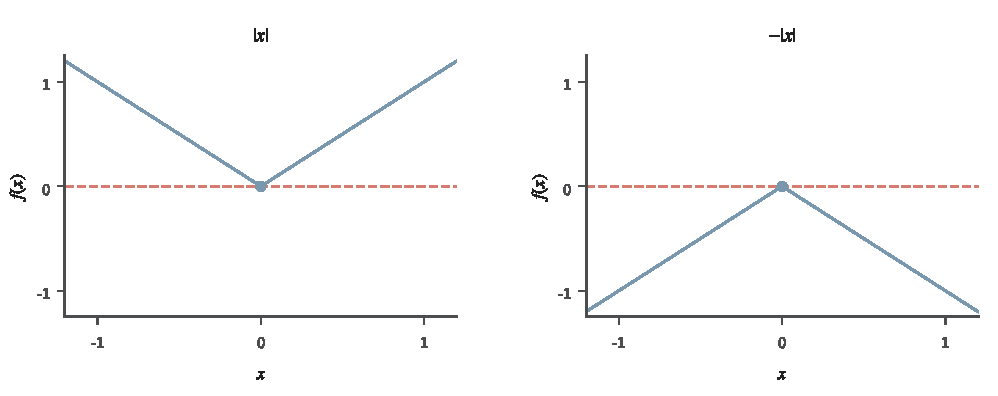
\includegraphics[width=\linewidth]{figures/01-mathematical-preliminaries/01-mathematical-language-combinatorics-analysis-optimization/matplotlib/teaching-analysis/analysis-clarke-stationarity-boundary.pdf}
 \caption{同一广义驻点条件的不同含义。蓝线分别为$|x|$与$-|x|$，红虚线为原点处候选斜率$g=0$对应的直线。
 两图在原点的Clarke广义梯度均为$[-1,1]$，却分别形成局部最小点与局部最大点；只有左图红线是全局仿射下界。
 两图共用坐标尺度，由解析式生成。}
 \label{fig:analysis-clarke-stationarity-boundary}
\end{figure*}



在含阈值或脉冲事件的模型中，常保留离散前向映射，却在反向计算时把其导数替换成某个平滑且非零的函数。这种信号称为\term{替代梯度}（surrogate gradient）。它是算法人为指定的近似更新方向，不自动等于前向映射的经典导数，也通常不满足凸次梯度的不等式。因此使用时应分别写清前向函数、反向替代函数及其尺度，不能把训练规则描述成对原离散函数的精确求导。

中心差分
\[   \frac{f(x+\varepsilon)-f(x-\varepsilon)}{2\varepsilon} \]
只能检验实际代入的函数$f$在尺度$\varepsilon$附近怎样变化。若程序反向传播使用替代梯度，而数值差分计算离散前向函数，两者本来就不是同一个导数对象；不一致不必然说明程序实现错误。

\section{函数的可测性与整体关系}
\label{sec:analysis-integration-average}

局部变化研究一个位置附近的输出增量；整体累计还要知道每个范围占多少权重。
第~\ref{sec:analysis-set-structures}节已建立可测集合族与测度，现在把函数的取值
与这些范围连接起来：可测性保证按取值分组后仍能赋权，积分再把每组贡献累计为总量。
整体关系还包括变量之间怎样共同累计，以及局部导数怎样转化为边界贡献。

\subsection{函数的可测性}

测度只知道集合的大小，还不知道函数在集合上贡献多少。把函数按取值分组后，每组
贡献就是“该取值乘以这组的测度”。因此，在写积分之前，要保证这些取值集合属于
已经允许测量的范围。

可测性说的是函数与这些测量范围是否相容：对输出值提出一个可测的条件，满足条件的
输入也应组成可测集合。这里需要的是集合的原像，并不要求函数有逆函数。
\begin{definition}[可测函数]
\label{def:analysis-measurable-function}
给定可测空间$(X,\mathcal{A})$与$(Y,\mathcal{B})$。若映射$f:X\to Y$满足
\[
  B\in\mathcal{B}\quad\Longrightarrow\quad
  f^{-1}(B)=\{x\in X:f(x)\in B\}\in\mathcal{A},
\]
则称$f$为从$(X,\mathcal{A})$到$(Y,\mathcal{B})$的\term{可测函数}
（measurable function）。对取值于$\mathbb{R}$或$\overline{\mathbb{R}}=[-\infty,\infty]$
的函数，目标空间取Borel $\sigma$代数；此时可测性等价于
\[
  \{x\in X:f(x)>a\}\in\mathcal{A}
  \qquad\text{对每个 }a\in\mathbb{R}\text{成立}.
\]
\end{definition}
阈值条件之所以足够，是因为这些半直线能生成目标空间的Borel $\sigma$代数，而原像
保持补集与可数并。它保证按函数值分层得到的集合都能取得测度。可测性依赖指定的
$\sigma$代数，并不依赖这些集合具体有多大权重。例如在$X=\{a,b\}$上只允许
$\mathcal{A}=\{\varnothing,X\}$时，$f(a)=0$、$f(b)=1$不可测：阈值$1/2$选出
$\{b\}$，不在$\mathcal{A}$中。把$\mathcal{A}$改为所有子集后，同一个函数就可测。

连续性比较输入与输出的距离，本身不以可测性为先决条件。若两端采用Borel $\sigma$代数，连续映射自动可测，因为开集的原像仍是开集；若任意指定其他$\sigma$代数，则不能只凭连续性保证可测。反向也不成立。
例如$[0,1]$上有理数的指示函数$\mathbb{I}_{\mathbb{Q}\cap[0,1]}$可测，因为有理数
集合是可数个单点的并，但它在每一点都不连续：任意小邻域内同时有有理数和无理数，
函数值在$1$和$0$之间跳变。可测性只保证取值分组可以测量，不保证图像平滑，
也不保证积分有限。可测函数列的逐点极限存在时仍可测，可数族可测函数的逐点上确界
和下确界也可测。这些封闭性使下面的阶梯逼近能够留在同一套积分框架中。

这些极限的可测性可以直接回到集合运算，而不依赖尚未建立的积分定理。对可测实函数列，
\begin{align*}
 \{x:\sup_n f_n(x)>a\}&=\bigcup_n\{x:f_n(x)>a\},\\
 \{x:\inf_n f_n(x)<a\}&=\bigcup_n\{x:f_n(x)<a\}.
\end{align*}
因此上确界、下确界可测；再用
$\liminf_n f_n=\sup_N\inf_{n\geq N}f_n$，得到下极限可测，逐点极限存在时就是它。
有限加法、绝对值、最大值等连续运算也保持实函数的可测性：
$(f,g)$的矩形原像是两个可测原像的交，而实平面的开集可写成可数个有理端点矩形的并。
这为后面按$\{f>a\}$分层、取正负部分和比较$f,g$提供了集合依据。

例如在$X=\mathbb R$上采用通常距离，却只允许
$\mathcal A=\{\varnothing,\mathbb R\}$，目标采用Borel集合族，则连续函数$f(x)=x$
不是从$(X,\mathcal A)$到目标可测空间的可测函数：开区间$(0,1)$的原像不属于
$\mathcal A$。因此可测、连续与可积需要分别核对其结构与条件。
即使固定Lebesgue测度，连续也不等于可积：$f(x)=1/x$在$(0,1)$上连续且可测，
总积分却为无穷。相反，有理数指示函数虽处处不连续，积分却为零。
下面构造积分后，再核对这些大小关系；可测性负责“能否按取值赋权”，可积性负责
“绝对贡献是否有限”。

\subsection{积分的构造与可积性}
\subsubsection{简单函数与非负积分}
一般函数可能取无穷多个不同的值，先从只取有限多个值的可测函数开始。它们可以按
每个取值对应的集合分组，使积分直接退化为有限加权和。
\begin{definition}[简单函数及其积分]
\label{def:analysis-simple-function-integral}
在可测空间$(X,\mathcal{A})$上，只取有限多个实数值的可测函数称为
\term{简单函数}（simple function）。非负简单函数可以表示为
\[   s(x)=\sum_{j=1}^{m}a_j\mathbb{I}_{A_j}(x),   \qquad a_j\in[0,\infty),\quad A_j\in\mathcal{A}, \]
其中$A_j$两两不交，$\mathbb{I}_{A_j}$在$A_j$上取$1$、其余处取$0$。
给定测度$\mu$，其积分定义为
\begin{equation}
  \int_X s\,\mathrm{d}\mu
  =
  \sum_{j=1}^{m}a_j\mu(A_j).
\label{eq:analysis-simple-integral}
\end{equation}
约定$0\cdot\infty=0$，并允许积分取$+\infty$。
\end{definition}
同一个简单函数可能有不同的分组表示；把这些表示按所有取值集合的交集细分成共同的
两两不交集合后，有限可加性给出相同的和，因此式~\eqref{eq:analysis-simple-integral}
不依赖具体表示。
同样的共同细分还给出简单函数的大小关系与非负线性：
若$s\leq t$，则$\int s\leq\int t$；若$\alpha,\beta\geq0$，则
$\int(\alpha s+\beta t)=\alpha\int s+\beta\int t$。
这些结论只涉及同一组可测块上的有限加权和，尚未对一般函数交换极限和积分。

例如对$[0,1]$上的$f(x)=x$，用两段阶梯从下方近似：前半段取$0$，后半段取
$1/2$，其积分为$1/4$。细分成四段并取每段左端点的函数值，积分变成
$(0+1/4+1/2+3/4)/4=3/8$；继续细分，阶梯越来越接近原函数，面积趋于熟悉的$1/2$。
这里每个阶段都只计算有限个“取值$\times$集合长度”，极限才把它们接成一般积分。

这一做法不限于区间。每个非负可测函数$f$都能由一列非负简单函数从下方逐点逼近。
对$n\geq1$，一个明确的构造是
\begin{equation}
  s_n(x)
  =
  \sum_{k=0}^{n\,2^n-1}
  \frac{k}{2^n}
  \mathbb{I}_{\{k\,2^{-n}\leq f(x)<(k+1)2^{-n}\}}
  +
  n\mathbb{I}_{\{f(x)\geq n\}}.
\label{eq:analysis-canonical-simple-approximation}
\end{equation}
它先把函数值截断在$n$，再向下舍入到间距为$2^{-n}$的格点。截断高度随$n$增加，
格点也逐次细化，所以$0\leq s_n\leq s_{n+1}\leq f$。若$f(x)<\infty$，当
$n>f(x)$时还有$0\leq f(x)-s_n(x)<2^{-n}$；若$f(x)=+\infty$，则
$s_n(x)=n$。因此$s_n(x)\uparrow f(x)$对每个$x$成立。每个下方阶梯给出一个不超过
真实总量的值；把所有这种值的上界收紧，就得到非负积分。
图~\ref{fig:analysis-simple-integral}把同一构造用于$f(x)=x^2$。等距划分的是
\emph{函数值}，对应的输入区间宽度不必相等；每块黄色面积仍是一个取值乘以
它的原像集合的测度。随着取值间距缩小，下方阶梯留下的空隙逐渐减小。
\begin{figure*}[htbp]
 \centering
 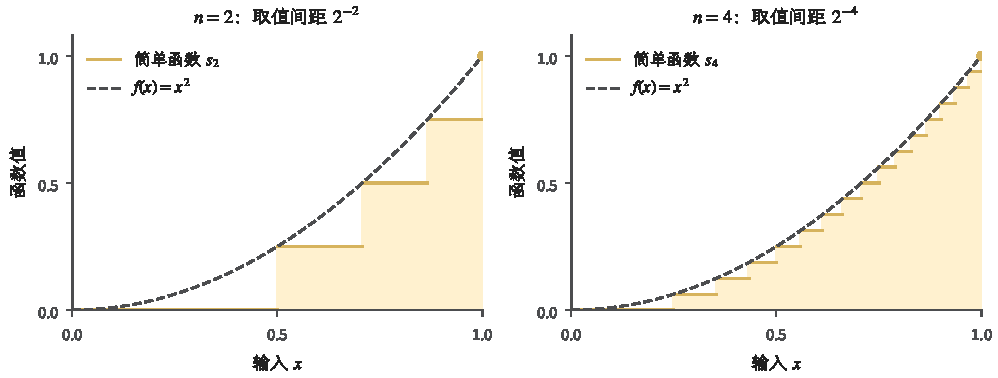
\includegraphics[width=\linewidth]{figures/01-mathematical-preliminaries/01-mathematical-language-combinatorics-analysis-optimization/matplotlib/concepts-analysis-functional/simple-integral.pdf}
 \caption{按取值分层的简单函数逼近。两图都使用式~\eqref{eq:analysis-canonical-simple-approximation}的构造，分别取$n=2$和$n=4$；本例中高度截断不起作用。黄色阶梯下的面积是有限加权和，目标曲线下的面积为$1/3$。两图共用坐标尺度。}
 \label{fig:analysis-simple-integral}
\end{figure*}
\begin{definition}[非负函数的Lebesgue积分]
\label{def:analysis-nonnegative-lebesgue-integral}
在测度空间$(X,\mathcal{A},\mu)$上，非负可测函数$f:X\to[0,\infty]$的积分定义为
\begin{equation}
  \int_X f\,\mathrm{d}\mu
  =
  \sup\left\{
    \int_X s\,\mathrm{d}\mu:
    0\leq s\leq f,\ s\text{为简单函数}
  \right\}.
\label{eq:analysis-nonnegative-lebesgue-integral}
\end{equation}
这里允许结果为$+\infty$。
\end{definition}
这个定义不要求把定义域切成连续小区间，而是按函数值分层，所以能自然处理极限和
零测例外。式~\eqref{eq:analysis-canonical-simple-approximation}给出的阶梯也可用来
计算这个上确界；下面的单调收敛定理说明，任意这样的递增逼近都能计算这个上确界。

\subsubsection{单调逼近与积分性质}
非负积分定义直接保留大小关系：若$0\leq f\leq g$，每个不超过$f$的简单函数
也不超过$g$，所以$\int f\,\mathrm d\mu\leq\int g\,\mathrm d\mu$。
它也继承零测修改不变性。设$N$可测且$\mu(N)=0$，$f,g$可测非负并在$X\setminus N$
相等。任取简单函数$0\leq s\leq f$，去掉$N$上的部分得到
$s\mathbb I_{X\setminus N}\leq g$，且简单函数积分没有改变；取上确界得到
$\int f\leq\int g$，反向同理。这里没有用一般积分的线性，只用了简单函数的有限和。
修改后的函数仍须可测；在未完备测度空间中，不能在零测集上任意修改而省略这项要求。

一种防止总量在逼近中消失的方式，是只让非负贡献逐步增加。它正好对应上面的下方阶梯。记$f_n(x)\uparrow f(x)$表示每个固定$x$处的数列单调增加且趋于$f(x)$；允许忽略零测例外时，例外须包含在同一个可测零测集中。下面把阶梯逼近推广到任意递增的非负可测函数列\scite{math-folland1999real}
\begin{theorem}[单调收敛定理]
\label{thm:analysis-monotone-convergence}
设$f_n,f:X\to[0,\infty]$可测，且$f_n(x)\uparrow f(x)$几乎处处，则
\[   \lim_{n\to\infty}\int_X f_n\,\mathrm{d}\mu   =   \int_X f\,\mathrm{d}\mu. \]
两边都允许取$+\infty$。
\end{theorem}
\begin{proof}
把单调性或收敛关系失效的可测零测集并为$N$，并将$f_n$与$f$在$N$上都改为$0$。
修改后的函数仍可测且积分不变，所以可假定$f_n\uparrow f$逐点成立。由
$0\leq f_n\leq f$，积分序列单调不减且
\[   L:=\lim_{n\to\infty}\int f_n\,\mathrm{d}\mu   \leq\int f\,\mathrm{d}\mu. \]
还需证明反向不等式。任取满足$0\leq s\leq f$的简单函数，将它写为 $s=\sum_{j=1}^m a_j\mathbb{I}_{E_j}$，其中$a_j>0$且$E_j$两两不交。固定 $c\in(0,1)$，定义
\[   E_{j,n}   =   E_j\cap\{x:f_n(x)\geq ca_j\}. \]
由于$f_n\uparrow f$且$f\geq a_j$于$E_j$，有$E_{j,n}\uparrow E_j$。
第~\ref{sec:analysis-set-measure-continuity}节已由可数可加性证明测度对递增集合连续，
故$\mu(E_{j,n})\uparrow\mu(E_j)$。同时
\[   f_n   \geq   c\sum_{j=1}^m a_j\mathbb{I}_{E_{j,n}}, \]
从而
\[   L   \geq   \lim_{n\to\infty}   c\sum_{j=1}^m a_j\mu(E_{j,n})   =   c\int s\,\mathrm{d}\mu. \]
先令$c\uparrow1$，再对所有$0\leq s\leq f$的简单函数取上确界。根据非负积分的定义~\eqref{eq:analysis-nonnegative-lebesgue-integral}， $L\geq\int f\,\mathrm{d}\mu$。与前一不等式合并即得结论。
\end{proof}

非负性避免正负无穷相消，单调性则保证已经积累的质量不会在后续消失。定理不要求存在一个可积的统一上界，也不要求各$\int f_n$有限。

单调收敛已经说明递增逼近怎样保留总量。积分还应继承有限和的两个基本规律：贡献增加时总量不能减少，非负线性组合的总量
等于各总量的同一线性组合。下面给出它们在一般测度空间中的版本；证明的任务是把
有限和的性质传到定义中的上确界，不能仅凭熟悉的Riemann积分规则就跳过这一推广。
\begin{lemma}[非负积分的线性与单调性]
\label{lem:analysis-nonnegative-integral-properties}
设$f,g:X\to[0,\infty]$可测，$\alpha,\beta\geq0$。若$f\leq g$几乎处处，则
\[
  \int_X f\,\mathrm{d}\mu\leq\int_X g\,\mathrm{d}\mu.
\]
此外，在$0\cdot\infty=0$的约定下，
\[
  \int_X(\alpha f+\beta g)\,\mathrm{d}\mu
  =
  \alpha\int_X f\,\mathrm{d}\mu
  +
  \beta\int_X g\,\mathrm{d}\mu.
\]
\end{lemma}
\begin{proof}
对$f\leq g$几乎处处的情形，集合$N=\{x:f(x)>g(x)\}$可测且$\mu(N)=0$。把$f$在
$N$上改为$0$得到可测函数$\widetilde f$，其积分与$f$相同，并且逐点满足
$\widetilde f\leq g$。此时每个满足$0\leq s\leq\widetilde f$的简单函数也满足
$s\leq g$；
在式~\eqref{eq:analysis-nonnegative-lebesgue-integral}中取上确界便得到单调性。

还需把简单函数的线性提升到一般非负函数。前面的单调收敛定理
\ref{thm:analysis-monotone-convergence}已保证：非负可测函数递增逼近其极限时，
积分也递增趋于极限的积分。现在分别取
非负简单函数$s_n\uparrow f$和$t_n\uparrow g$，则
$\alpha s_n+\beta t_n\uparrow\alpha f+\beta g$。对这三个函数列应用单调收敛定理，
结合简单函数的线性性，即得
\[
  \int_X(\alpha f+\beta g)\,\mathrm{d}\mu
  =
  \lim_{n\to\infty}
  \left(
    \alpha\int_Xs_n\,\mathrm{d}\mu
    +
    \beta\int_Xt_n\,\mathrm{d}\mu
  \right),
\]
右侧正是结论中的两个积分之和。
\end{proof}

简单函数的共同细分在单调收敛之前建立，一般函数的线性则在单调收敛之后建立；
两者不能倒置。对任意可测非负函数列$u_k$，再把线性用于有限部分和并用单调收敛，
还得到$\int\sum_{k\geq1}u_k=\sum_{k\geq1}\int u_k$，允许两边为无穷。
例如$(0,\infty)$上的$\mathbb I_{(0,n)}\uparrow1$，积分从$n$增至无穷；
单调收敛并不承诺最终总量有限。

\subsubsection{有符号积分与可积性}

非负函数只累积贡献，允许总量为$+\infty$。含正负值的函数却可能一边累积
$+\infty$、另一边累积$-\infty$，不能用二者相消来定义一个数。因此先把正、负贡献
分别计算，再决定它们是否允许相减。
\begin{definition}[有符号积分与可积性]
\label{def:analysis-integrable-function}
在测度空间$(X,\mathcal{A},\mu)$上，对可测实函数$f$，令
\[   f^+(x)=\max\{f(x),0\},\qquad   f^-(x)=\max\{-f(x),0\}. \]
若$\int_X f^+\,\mathrm{d}\mu$与$\int_X f^-\,\mathrm{d}\mu$不同时为无穷，则定义
\[
  \int_X f\,\mathrm{d}\mu
  =\int_X f^+\,\mathrm{d}\mu-\int_X f^-\,\mathrm{d}\mu.
\]
若
\begin{equation}
  \int_X|f|\,\mathrm{d}\mu<\infty,
\label{eq:analysis-absolute-integrability}
\end{equation}
就称$f$\term{绝对可积}（absolutely integrable）或Lebesgue可积。
\end{definition}
由于$f=f^+-f^-$且$|f|=f^++f^-$，可积性等价于正负两部分的积分都有限。
此时积分没有“无穷减无穷”的歧义，并满足
\[   \left|\int_X f\,\mathrm{d}\mu\right|   \leq   \int_X|f|\,\mathrm{d}\mu. \]

有符号线性也需要这项有限性。若$f,g$可积，$|f+g|\leq|f|+|g|$
先保证$f+g$可积。记$u=f+g$，由逐点恒等式
$u^++f^-+g^-=u^-+f^++g^+$，对两边的非负项积分并使用已证明的线性，
再移去有限项，得到$\int(f+g)=\int f+\int g$。
非负常数倍由前面的引理处理，负常数倍则交换正负部分，所以
$\int(\alpha f+\beta g)=\alpha\int f+\beta\int g$对任意实数$\alpha,\beta$成立。
若$f\leq g$几乎处处，对非负函数$g-f$积分还得到$\int f\leq\int g$。

在闭区间上有界且Riemann可积的函数也Lebesgue可积，两种积分取值相同。Lebesgue积分
并非否定熟悉的面积解释，而是扩大可处理的函数，并让两个可测且几乎处处相等的函数
具有相同积分。例如在Lebesgue测度下，修改可测函数在单点上的值仍得到可测函数，也不
改变积分。反过来，积分有限不表示函数处处有界，也不自动给出连续性。
例如在$(0,1)$上，$x^{-1/2}$无界却可积：对
$x^{-1/2}\mathbb I_{[1/n,1)}$用闭区间上的熟悉积分，再用单调收敛，得到
$\int_0^1x^{-1/2}\,\mathrm dx=\lim_n2(1-n^{-1/2})=2$。
而对$x^{-1}$同样计算得到$\lim_n\log n=+\infty$；它的非负积分有定义，
却不是可积函数。若在$(-1,1)$取$f(x)=1/x$（原点取$0$），正负部分积分都为无穷，
Lebesgue积分便没有定义。对称截断得到的零是另一种极限约定，不能替代这里的积分。

有限集合上的积分就是带测度权重的求和。回到第~\ref{sec:analysis-set-structures}节的$X=\{a,b\}$，
$\mu(\{a\})=1$、$\mu(\{b\})=2$，并令$f(a)=3$、$f(b)=-1$。则
\[
 \int_Xf\,\mathrm d\mu=3\times1+(-1)\times2=1,
 \qquad \int_X|f|\,\mathrm d\mu=5.
\]
积分是总量；若要把它称为平均，还要除以总质量$\mu(X)=3$，得到$1/3$。
概率测度的总质量为$1$，才无需这一步归一化。这个小例子也显示，正负部分可以相消，
可积性却要分别控制它们的大小。
一般地，按$\mu$取一个有限平均要求$f$可积且$0<\mu(X)<\infty$，此时平均为
$\mu(X)^{-1}\int_X f\,\mathrm d\mu$。总质量为零时不能相除，总质量无穷时也不能把
有限积分除以无穷来定义这项平均；需要另行指定局部区域或归一化方式。

\subsection{乘积积分与次序交换}

前面讨论的是一个位置$x$上的贡献；若函数同时依赖$x$和$y$，就要给成对位置
$(x,y)$所在的集合赋权重。对两组分别给定的权重，最自然的扩展是让矩形
$A\times B$的权重等于两边权重的乘积。它是面积“长乘宽”以及有限双重加权和的
共同推广，称为乘积测度。

为了由矩形权重唯一确定一般集合的权重，下面采用一种常见条件：整个空间可以由
可数个有限权重的区域覆盖。这比要求空间的总权重有限宽松，例如整个实数轴长度无限，
却能写成区间$[-n,n]$的并。
\begin{definition}[$\sigma$有限测度]
\label{def:analysis-sigma-finite-measure}
若存在$E_n\in\mathcal{A}$，使$X=\bigcup_{n=1}^{\infty}E_n$且对每个$n$有
$\mu(E_n)<\infty$，称测度空间$(X,\mathcal{A},\mu)$是
\term{$\sigma$有限}（sigma-finite）的。
\end{definition}
例如$\mathbb N$上的计数测度可由有限集合$\{1,\ldots,n\}$覆盖，因而$\sigma$有限；
不可数集合上的计数测度则不满足这一条件，因为可数个有限集合的并仍然可数。
所以“每个点质量有限”远弱于“整个空间能由可数个有限质量区域覆盖”。

在两个$\sigma$有限测度空间上，乘积测度定理保证：矩形上的乘积权重能扩展为一个
存在且唯一的测度。下面用这一性质刻画它。
\begin{definition}[乘积$\sigma$代数与乘积测度]
\label{def:analysis-product-measure}
给定两个$\sigma$有限测度空间$(X,\mathcal{A},\mu)$与$(Y,\mathcal{B},\nu)$。
包含所有矩形$A\times B$（$A\in\mathcal{A}$，$B\in\mathcal{B}$）的最小
$\sigma$代数称为乘积$\sigma$代数，记为$\mathcal{A}\otimes\mathcal{B}$。
在该$\sigma$代数上，对任意这样的$A,B$满足
\[   (\mu\otimes\nu)(A\times B)=\mu(A)\nu(B) \]
的测度记为$\mu\otimes\nu$，称为\term{乘积测度}（product measure）。
这里仍约定$0\cdot\infty=0$。
\end{definition}
对矩形上的指示函数，先对$x$积分或先对$y$积分都得到同一个乘积。一般函数能否继续交换积分次序，则取决于非负性或绝对可积性，下面给出准确条件。若脱离$\sigma$有限框架，乘积测度的唯一性和相应积分结论需要
更谨慎的版本。

有限网格把这个构造还原为双重求和。若$X=\{x_1,\ldots,x_m\}$、
$Y=\{y_1,\ldots,y_n\}$分别带权重$u_i,v_j$，则
\[
  \int_{X\times Y}f\,\mathrm{d}(\mu\otimes\nu)
  =
  \sum_{i=1}^m\sum_{j=1}^n f(x_i,y_j)u_iv_j.
\]
有限和可以直接交换次序；一般测度空间中的累次积分还要处理无穷值与极限，
不能只由矩形公式推出。还要注意，乘积测度是一种特定构造；一般的二元概率分布
可以包含两个变量之间的依赖，并不必然等于两边概率测度的乘积。第~\ref{chap:probability-theory}章会
在联合分布与独立性的语境中回用这一区别。

乘积测度确定成对位置的权重，尚未保证任意函数都能按两个次序分别累计。这里比较累次积分与乘积空间上的积分：非负性允许逐步累计，绝对可积性排除正负无穷相消；刚建立的单调收敛把简单函数的累计规则推广到一般非负函数。
\begin{theorem}[Tonelli与Fubini定理]
\label{thm:analysis-tonelli-fubini}
设$(X,\mathcal{A},\mu)$与$(Y,\mathcal{B},\nu)$为$\sigma$有限测度空间，且 $f:X\times Y\to\overline{\mathbb{R}}$对乘积$\sigma$代数可测。
\begin{itemize}

\item 若$f\geq0$，则每个截面$y\mapsto f(x,y)$与$x\mapsto f(x,y)$都可测，并且两个
  内层积分函数
  \[
    x\longmapsto\int_Yf(x,y)\,\mathrm{d}\nu(y),
    \qquad
    y\longmapsto\int_Xf(x,y)\,\mathrm{d}\mu(x)
  \]
  分别关于$x$与$y$可测，且
  \[
    \begin{aligned}
      \int_{X\times Y}f\,\mathrm{d}(\mu\otimes\nu)
      &=
      \int_X\left(\int_Yf(x,y)\,\mathrm{d}\nu(y)\right)\mathrm{d}\mu(x)\\
      &=
      \int_Y\left(\int_Xf(x,y)\,\mathrm{d}\mu(x)\right)\mathrm{d}\nu(y).
    \end{aligned}
  \]
  允许共同值为$+\infty$。这是Tonelli定理。
\item 若$\int_{X\times Y}|f|\,\mathrm{d}(\mu\otimes\nu)<\infty$，则
  $y\mapsto f(x,y)$对几乎每个$x$可积，$x\mapsto f(x,y)$对几乎每个$y$可积。
  把相应内层积分函数在例外集上置为$0$后，它们分别可积，上述等式对$f$成立并取有限值。
  这是Fubini定理。
\end{itemize}
\end{theorem}

证明可分为集合与函数两层。对矩形指示函数$\mathbb I_{A\times B}$，三种积分都等于
$\mu(A)\nu(B)$；有限可加性把这个结论扩展到有限分割形成的集合。
从这些集合进入乘积$\sigma$代数中的\emph{任意}可测集合，还需要测度论的扩张论证，
不是仅靠每个矩形上的等式便能完成；完整论证见所引测度论教材
\scite{math-folland1999real}
本章关注扩张之后的函数层：指示函数的结论经线性组合进入非负简单函数，再经
$s_n\uparrow f$和单调收敛进入任意非负可测函数，得到Tonelli。
若$f$绝对可积，则对$f^+$和$f^-$分别应用Tonelli；绝对积分有限保证两部分不会
出现无穷减无穷，相减才得到Fubini。这里给出证明的依赖路线，不把矩形核对当作
完整证明。

这里非负性允许无穷值，绝对可积性则排除了依赖积分次序的条件相消。例如在
$\mathbb{N}\times\mathbb{N}$上使用计数测度时，Tonelli说明非负双重级数可以任意交换
求和次序；Fubini说明绝对收敛的双重级数也可以这样做。若既不非负也不绝对可积，
交换次序可能改变结果，甚至一个次序收敛而另一个发散。因此“把两个积分换一下”
不是排版操作，而是需要先核对函数符号或绝对积分的数学步骤。

\begin{example}[行列各自可加仍不足以换序]
\label{ex:analysis-iterated-sum-failure}
在$\mathbb N\times\mathbb N$上令
$a_{i,j}=\mathbb I\{j=i\}-\mathbb I\{j=i+1\}$，两边均用计数测度。
每一行只有一个$1$和一个$-1$，故$\sum_j a_{i,j}=0$；
第一列的和为$1$，其余每一列的和为$0$。于是
\[
 \sum_{i=1}^{\infty}\left(\sum_{j=1}^{\infty}a_{i,j}\right)=0,
 \qquad
 \sum_{j=1}^{\infty}\left(\sum_{i=1}^{\infty}a_{i,j}\right)=1.
\]
两种累次和都有有限值，却不相等。每行的绝对值和为$2$，所以整个绝对积分为无穷，
正负部分也各为无穷。失效的是Fubini的绝对可积条件，而非某一行的计算规则。
\end{example}

$\sigma$有限也有实际作用。在$[0,1]$上让$x$采用Lebesgue测度、$y$采用
不可数集合上的计数测度，取非负函数$f(x,y)=\mathbb I\{x=y\}$。
对角线属于乘积$\sigma$代数，但先对$y$计数再对$x$积分得到$1$，
先对$x$求长度再对$y$计数却得到$0$。这里不满足本章Tonelli版本的$\sigma$有限条件，
不能只凭非负性换序。

\subsection{积分换元与坐标变换}
\label{sec:analysis-coordinate-change-integral-applications}
积分的定义、权重和可积条件已经确定，现在可以利用函数或区域的结构计算它。
换元重新表示同一个区域，函数值要随坐标复合，每块区域的体积权重也要随之修正。
链式法则中的Jacobian把一个输入扰动映成输出扰动；这里则需要把多个方向共同张成的
体积缩放成一个非负权重，起作用的是Jacobian行列式的绝对值。

一维换元中，$u=T(x)$把长度$\mathrm{d}x$缩放为约 $|T'(x)|\mathrm{d}x$。在$d$维，局部线性近似
\[   T(\bm{x}+\bm{h})   \approx   T(\bm{x})+\bm{J}_T(\bm{x})\bm{h} \]
把一个小平行多面体的有向体积乘以 $\det\bm{J}_T(\bm{x})$，普通体积则乘以其绝对值。行列式为零意味着至少一个方向被压扁，局部逆映射通常不再存在。

设$U,V\subseteq\mathbb{R}^d$为开集， $T:U\to V$是连续可微双射，逆映射也连续可微，并且 $\det\bm{J}_T(\bm{x})\neq0$。对非负可测函数或绝对可积函数$g$，多维换元公式为
\begin{equation}
  \int_V g(\bm{y})\,\mathrm{d}\bm{y}
  =
  \int_U
  g\bigl(T(\bm{x})\bigr)
  \left|\det\bm{J}_T(\bm{x})\right|
  \,\mathrm{d}\bm{x}.
\label{eq:analysis-multivariate-change-variables}
\end{equation}
绝对值不可省略，因为积分中的体积不随坐标方向翻转而变成负数。一维单调换元是 $d=1$的特例；若在定积分中保留有向上下限，也可让导数符号由上下限次序吸收。
公式的证明可理解为把$U$分成足够小的区域：在每一块上用
$T(\bm{x}+\bm{h})\approx T(\bm{x})+\bm{J}_T(\bm{x})\bm{h}$替代原映射，
线性映射把该块体积乘以$|\det\bm{J}_T(\bm{x})|$，再让分割尺度趋于零。
这条路线只提供直观框架；严格证明还要控制局部近似误差、像集重叠和可测逼近，
不能把逐点线性化直接当作全局换元等式。
\begin{example}[极坐标中的面积权重]
\label{ex:analysis-polar-coordinate-jacobian}
令$D=\{\bm{x}\in\mathbb{R}^2:\lVert\bm{x}\rVert_2\leq1\}$，并令
$T(r,\theta)=(r\cos\theta,r\sin\theta)$。在开集
$(0,1)\times(0,2\pi)$上，$T$是到开圆盘内部去掉原点和正$x$轴径向接缝后的区域的
连续可微双射，逆映射也连续可微。其Jacobian矩阵的行列式为
\[   \det
\begin{bmatrix}     \cos\theta & -r\sin\theta\\     \sin\theta & r\cos\theta
\end{bmatrix}   =r. \]
圆周、原点和径向接缝都是二维零测集；参数矩形的边界也是零测集。因此在上述开集上应用
换元公式，再补回这些零测部分，便得到
\[   \int_D1\,\mathrm{d}\bm{x}   =   \int_0^{2\pi}\int_0^1r\,\mathrm{d}r\,\mathrm{d}\theta   =\pi. \]
这里积分上下限包含端点不改变积分值。若参数化在正测度区域上重复覆盖，则不能直接使用
上述双射版本，否则同一点会被重复计数。
\end{example}
\subsection{微分与积分的关系}

换元改变坐标表示，以下公式则把局部变化的累计与端点或边界联系起来。
一维乘积求导产生分部积分，沿曲线的链式求导产生端点差，区域中的流出率则对应边界通量。
三种关系采用不同的积分对象，不能省去各自的端点、方向或面积权重。

\subsubsection{分部积分与积分余项}
\label{sec:analysis-integration-remainders}

先回顾微积分基本定理的连续版本。若$g$在$[a,b]$上连续，
$H(x)=\int_a^xg(t)\,\mathrm dt$在内点处满足$H'(x)=g(x)$；
若$H\in C^1([a,b])$，则$\int_a^bH'(x)\,\mathrm dx=H(b)-H(a)$。
这里$C^1$表示一阶连续可微，在闭区间端点采用单侧导数的连续延拓。
第一条可由
$[H(x+h)-H(x)]/h-g(x)=h^{-1}\int_x^{x+h}(g(t)-g(x))\,\mathrm dt$
和连续性得到；第二条再对$H(x)-H(a)-\int_a^xH'(t)\,\mathrm dt$
使用零导数蕴含常值的中值定理。这说明所用的是连续导数的积分，不是
“几乎处处存在导数便能恢复函数”的无条件结论。

有些乘积的积分难算，但把导数转移到另一个因子后会简化。分部积分就是这种转移规则，代价是增加边界贡献。若$u,v\in C^1([a,b])$，由乘积求导$(uv)'=u'v+uv'$并在$[a,b]$上积分，可得
\begin{equation}
  \int_a^b u(x)v'(x)\,\mathrm{d}x
  =
  [u(x)v(x)]_a^b
  -
  \int_a^b u'(x)v(x)\,\mathrm{d}x.
\label{eq:analysis-integration-by-parts}
\end{equation}
例如，取$u(x)=x$、$v'(x)=e^x$，得到 $\int_0^1xe^x\,\mathrm{d}x=[xe^x]_0^1-\int_0^1e^x\,\mathrm{d}x=1$。边界项不能无故删除；只有在函数于边界消失、区域无边界，或衰减速度足以使无穷远边界项趋零时才能省略。

分部积分还能把第~\ref{sec:analysis-taylor-approximation}节的局部二阶变化累计成有限位移的
余项。设连接$\bm{x}$与$\bm{x}+\bm{h}$的线段包含在一个开集内，且$f$在该开集上二阶
连续可微。令$\phi(t)=f(\bm{x}+t\bm{h})$，对$(1-t)\phi''(t)$在$[0,1]$上分部积分，得到
\[
  \int_0^1(1-t)\phi''(t)\,\mathrm{d}t
  =-\phi'(0)+\phi(1)-\phi(0).
\]
用链式法则代回，便得到不挑选中间点的Taylor积分余项：
\[   f(\bm{x}+\bm{h})   =   f(\bm{x})   +\nabla f(\bm{x})^{\top}\bm{h}   +   \int_0^1(1-t)   \bm{h}^{\top}\nabla^2f(\bm{x}+t\bm{h})\bm{h}\,\mathrm{d}t. \]
权重$1-t$说明越靠近位移起点的曲率贡献被累计得越多；该表达式与前面的中间点余项
描述同一有限变化，但保留了整条线段上的曲率信息。

一般阶数也由同一操作得到。设$f$在连接$x_0$和$x_0+h$的线段邻域内
$r+1$阶连续可微，$r\geq0$，令$\phi(t)=f(x_0+th)$。
记
\[
 I_r=\frac1{r!}\int_0^1(1-t)^r\phi^{(r+1)}(t)\,\mathrm dt.
\]
基本定理给出$I_0=\phi(1)-\phi(0)$；对$r\geq1$分部积分，
\[
 I_r=-\frac{\phi^{(r)}(0)}{r!}
       +\frac1{(r-1)!}\int_0^1(1-t)^{r-1}\phi^{(r)}(t)\,\mathrm dt
     =-\frac{\phi^{(r)}(0)}{r!}+I_{r-1}.
\]
逐次代入并用$\phi^{(k)}(0)=h^k f^{(k)}(x_0)$，便得
\begin{equation}
 f(x_0+h)=\sum_{k=0}^r\frac{f^{(k)}(x_0)}{k!}h^k
 +\frac{h^{r+1}}{r!}
   \int_0^1(1-t)^r f^{(r+1)}(x_0+th)\,\mathrm dt.
\label{eq:analysis-taylor-integral-remainder}
\end{equation}
参数化$x_0+th$同时处理正、负$h$。若$|f^{(r+1)}|\leq M$，积分权重的总量为
$1/(r+1)$，故余项不超过$M|h|^{r+1}/(r+1)!$，与前面的中间点余项界一致。
例如立方函数在$r=2$时有$f'''=6$，余项就是
$(h^3/2)\int_0^1 6(1-t)^2\,\mathrm dt=h^3$。
多元函数沿$\phi(t)=f(\bm x+t\bm h)$使用同一公式；$r=1$便还原前述Hessian积分余项。

\subsubsection{路径积分与端点关系}

换元仍是在同维区域内计算体积积分；如果贡献只沿一条路径累积，就应改用弧长或带方向的路径增量，不能继续套用全空间体积权重。设分段连续可微路径$\gamma:[a,b]\to\mathbb{R}^d$。对沿路径连续的标量函数
$h:\mathbb{R}^d\to\mathbb{R}$，标量线积分定义为
\[
  \int_\gamma h\,\mathrm{d}s
  =
  \int_a^b h(\gamma(t))\lVert\gamma'(t)\rVert_2\,\mathrm{d}t.
\]
速度的范数把参数增量换成弧长，因此反转路径方向不改变该积分。对沿路径连续的向量场
$\bm{F}:\mathbb{R}^d\to\mathbb{R}^d$，向量场线积分则定义为
\[   \int_{\gamma}\bm{F}\mathbin{\cdot}\mathrm{d}\bm{r}   =   \int_a^b   \bm{F}(\gamma(t))^{\top}\gamma'(t)\,\mathrm{d}t. \]
若$\bm{F}=\nabla\phi$且$\phi$连续可微，链式法则给出
\begin{equation}
  \int_{\gamma}\nabla\phi\mathbin{\cdot}\mathrm{d}\bm{r}
  =
  \phi(\gamma(b))-\phi(\gamma(a)).
\label{eq:analysis-line-integral-gradient}
\end{equation}
因此梯度场的路径积分只依赖端点。向量场线积分在路径方向反转时变号；若漏掉参数化导数
$\gamma'(t)$，就会丢失方向和行进速度的信息。

\begin{example}[同一路径上的长度、端点差与环流]
\label{ex:analysis-path-integral-comparison}
取单位圆的上半圆路径$\gamma(t)=(\cos t,\sin t)$，$0\leq t\leq\pi$。
它的速度范数恒为$1$，所以$\int_\gamma1\,\mathrm ds=\pi$。
取$\phi(x,y)=x$，则$\nabla\phi=(1,0)^\top$，
\[
 \int_\gamma\nabla\phi\mathbin{\cdot}\mathrm d\bm r
 =\int_0^\pi-\sin t\,\mathrm dt=-2
 =\phi(-1,0)-\phi(1,0).
\]
换成旋转场$\bm F(x,y)=(-y,x)^\top$时，
$\bm F(\gamma(t))^\top\gamma'(t)=1$，沿上半圆的积分为$\pi$。
但沿同样端点的直径路径$\eta(t)=(1-2t,0)$，$0\leq t\leq1$，
内积恒为零，积分为$0$。向量场连续甚至光滑，也不能单独保证路径无关。
沿完整单位圆逆时针一周，这个旋转场的积分为$2\pi$；梯度场沿闭合路径的端点差
必须为零，所以它不可能在整个平面上写成一个连续可微势函数的梯度。
\end{example}

\subsubsection{散度积分与边界通量}
路径积分沿行进方向累计，通量则计算穿过边界的贡献。在向量场
$\bm F=(F_1,\ldots,F_d)^\top$中，散度定义为
$\nabla\mathbin{\cdot}\bm F=\sum_{i=1}^d\partial F_i/\partial x_i$；
它把各坐标方向的局部流出率相加。相邻小区域的公共边界法向相反，
内部交换在总和中相消，剩下的应是外边界的净流出。

以下采用经典的规则区域版本：$\Omega$是有界开区域，其边界由有限个$C^1$
曲面片组成，每个光滑片附近区域位于边界的一侧，片间接缝的边界面积为零。
光滑区域、多边形和通常的多面体均符合这一条件。若向量场$\bm{F}$
在$\overline{\Omega}$的一个开邻域内连续可微，
\term{散度定理}（divergence theorem）写成
\begin{equation}
  \int_{\Omega}\nabla\mathbin{\cdot}\bm{F}\,\mathrm{d}\bm{x}
  =
  \int_{\partial\Omega}\bm{F}^{\top}\bm{n}\,\mathrm{d}S,
\label{eq:analysis-divergence-theorem}
\end{equation}
其中$\bm{n}$是外单位法向量，$\mathrm dS$表示边界上的面积元素。这个公式把区域内部与区域边界两种积分联系起来；左边汇总区域内部的局部流出率，右边计算穿过边界的净通量。它的严格适用条件随区域与函数空间版本而异；带尖点、无界区域或弱导数时，需要使用相应推广并重新核对边界项。分部积分、路径积分与散度定理共同说明，局部导数进入整体积分时， 通常会留下不可忽略的边界信息。

例如单位开圆盘$\Omega$上的$\bm F(x,y)=(x,y)^\top$有散度$2$，
故左边为$2\pi$。边界参数化$\gamma(t)=(\cos t,\sin t)$，$0\leq t\leq2\pi$，
外单位法向就是$\bm n=\gamma(t)$，弧长元素为$\mathrm dS=\mathrm dt$；
因此$\bm F^\top\bm n=1$，右边也为$2\pi$。
改用内法向会得到$-2\pi$，这不是同一定理中的方向约定。
前例的旋转场散度为零，且在圆周上始终与法向垂直，所以通量为零，
尽管沿切向的环流为$2\pi$。这一区别说明线积分和通量计算的不是同一种贡献。

\section{函数列的收敛与性质保持}
\label{sec:analysis-function-convergence-essential-bounds}

现在让被研究的函数本身随索引变化。$f_n:X\to\mathbb R$仍是一个序列，只是每一项
是函数；固定$x$以后，$f_n(x)$才成为第~\ref{sec:analysis-sequences-series-errors}节
的数值序列。比较整个函数还要选择误差尺度，并判断极限是否保留连续性、变化率或积分。
这些任务所需的基础不同：逐点收敛只需要数值极限，一致误差使用上确界，几乎处处
回用零测集，积分误差回用积分，导数逼近则回用第~\ref{sec:analysis-local-models}节
建立的局部变化信息。

\subsection{收敛方式与极限存在}
\subsubsection{逐点收敛与一致收敛}

固定一个输入以后，比较的只是一列实数。这里不需要函数可微或可积，甚至不需要
在输入集合上指定距离；函数值仍按实数绝对值比较。
\begin{definition}[逐点收敛]
\label{def:analysis-pointwise-almost-everywhere-convergence}
设$f_n,f:X\to\mathbb{R}$。若
\[
 \begin{gathered}
  \forall x\in X,\quad
  \forall\varepsilon>0,\quad
  \exists N=N(x,\varepsilon)\in\mathbb N,\\
  \forall n\geq N,\quad
  |f_n(x)-f(x)|<\varepsilon,
 \end{gathered}
\]
即对每个$x$都有$\lim_n f_n(x)=f(x)$，称$f_n$逐点收敛到$f$。
\end{definition}


定义中的每个位置都只比较一列实数；整体误差却不能靠分别检查各位置来控制。
即使每个输入处的误差最终都很小，开始稳定的时刻仍可能依赖输入。
若希望一次选定迭代次数后就控制全部输入，需要更强的一致条件。
\begin{definition}[函数列的一致收敛]
\label{def:analysis-uniform-convergence}
设$X$为非空集合，$f_n,f:X\to\mathbb R$。若
\[
  \forall\varepsilon>0,\quad
  \exists N=N(\varepsilon)\in\mathbb N,\quad
  \forall x\in X,\quad
  \forall n\geq N,\quad
  |f_n(x)-f(x)|<\varepsilon,
\]
就称$f_n$在$X$上一致收敛到$f$。等价地，
\begin{equation}
  \lVert f_n-f\rVert_{\infty}
  :=
  \sup_{x\in X}|f_n(x)-f(x)|
  \longrightarrow0.
\label{eq:analysis-uniform-convergence}
\end{equation}
这里的上确界检查全部输入，没有忽略零测集。
\end{definition}


两条定义的区别落在量词次序。逐点收敛允许$N$依赖$x$；一致收敛把$\exists N$
移到$\forall x$之前，同一个$N$必须同时控制全部输入。区别不在“趋近”这个词，
而在误差阈值之后允许谁依赖谁。下面用同一列函数比较这两种控制。

在$[0,1]$上取$f_n(x)=x^n$。它逐点收敛到
\[
 f(x)=
 \begin{cases}
  0,&0\leq x<1,\\
  1,&x=1.
 \end{cases}
\]
每个固定的$0<x<1$都有$x^n\to0$，而端点$1$的值始终为$1$。
但对每个$n$，$\sup_{0\leq x<1}x^n=1$，所以收敛不一致。
从量词看，固定$\varepsilon=1/2$后，无论选多大的$N$，在$n=N$时
总能选$x_N=(3/4)^{1/N}<1$，使误差$x_N^N=3/4>\varepsilon$。
失败的位置可以随$n$移动；不能把“每个位置最终变小”改写成“某一轮以后所有位置都小”。
若把范围缩为$[0,a]$，其中$a<1$，则上确界误差为$a^n\to0$，同一公式又变成一致收敛。

\subsubsection{几乎处处收敛与积分误差}

如果某些输入占零权重，是否必须在它们上面也逼近？积分任务通常不需要，
但必须先固定采用的测度和可忽略的范围。
\begin{definition}[几乎处处收敛]
\label{def:analysis-almost-everywhere-convergence}
给定测度空间$(X,\mathcal A,\mu)$和实函数$f_n,f$，若存在$E\in\mathcal A$、
$\mu(E)=0$，使
\[
 \forall x\in X\setminus E,\quad
 \forall\varepsilon>0,\quad
 \exists N=N(x,\varepsilon),\quad
 \forall n\geq N,\quad |f_n(x)-f(x)|<\varepsilon,
\]
就称$f_n$在$\mu$下几乎处处收敛到$f$。
\end{definition}
这里是先选一个零测集，再在它的补集上逐点收敛；每个精度和每一项不能任意丢掉
不同的正测度区域。可数个零测例外可以取并后统一，任意不可数个零测集的并却未必零测。
例如$x^n$关于$[0,1]$上的Lebesgue测度几乎处处趋于零，虽然它不在$x=1$处趋于零。
又如$f_n(x)=n\mathbb I_{\{0\}}(x)$几乎处处趋于零，但在$0$处连有限极限都没有。
若要求极限仍可测，本章采用各$f_n,f$均可测的版本；在未完备空间中，
不能从几乎处处关系自动推出任意指定的例外点取值可测。

如果关心的是按测度累计的误差，就要先说明被比较的函数属于什么空间。
积分不区分只在零测集上不同的可测函数：即使$f$不处处为零，$\int|f|^p\,\mathrm d\mu$
也可能为零。把这类函数视为同一个元素，才能让零误差对应空间中的同一个对象。
\Needspace{12\baselineskip}
\begin{definition}[$L^p$空间与范数]
\label{def:analysis-lp-space}
设$(X,\mathcal A,\mu)$为测度空间，$1\leq p<\infty$。对可测实函数定义等价关系
\[
  f\sim g\quad\Longleftrightarrow\quad f=g\text{在$\mu$下几乎处处成立}.
\]
$L^p(\mu)$由满足$\int_X|f|^p\,\mathrm d\mu<\infty$的可测实函数的等价类$[f]$组成，
其范数定义为
\[
  \lVert[f]\rVert_{L^p(\mu)}
  =\left(\int_X|f|^p\,\mathrm d\mu\right)^{1/p}.
\]
该值不依赖代表元的选择。下文用代表元$f$代写等价类$[f]$，并简记范数为
$\lVert f\rVert_p$。
\end{definition}

固定这个空间以后，函数列的收敛就可以由累计误差定义。
\begin{definition}[$L^p$收敛]
\label{def:analysis-lp-convergence}
设$1\leq p<\infty$，且$f_n,f\in L^p(\mu)$。若
\begin{equation}
  \lVert f_n-f\rVert_p
  :=
  \left(
    \int_X|f_n-f|^p\,\mathrm{d}\mu
  \right)^{1/p}
  \longrightarrow0,
  \qquad 1\leq p<\infty.
\label{eq:analysis-lp-convergence}
\end{equation}
就称$f_n$在$L^p(\mu)$中收敛到$f$。
\end{definition}
展开量词就是：对每个$\varepsilon>0$存在$N$，使所有$n\geq N$的
积分误差范数小于$\varepsilon$。这里受控的是整个积分，不是对每个$x$
分别要求$|f_n(x)-f(x)|<\varepsilon$。

回到上面的$f_n(x)=x^n$及其逐点极限$f$，对任意有限$p\geq1$，
\[   \lVert f_n-f\rVert_p^p   =   \int_0^1x^{np}\,\mathrm{d}x   =   \frac{1}{np+1}   \longrightarrow0. \]
同一函数列因此逐点且在每个有限$L^p$意义下收敛，却不一致收敛。区别来自最坏输入与累计误差采用了不同尺度。
图~\ref{fig:analysis-power-convergence-scales}把接近$x=1$的区域与误差数值并列。
每个固定的$x<1$最终都会下降，但每一轮总有更靠近$1$的新位置保留接近$1$的误差。
\begin{figure*}[htbp]
 \centering
 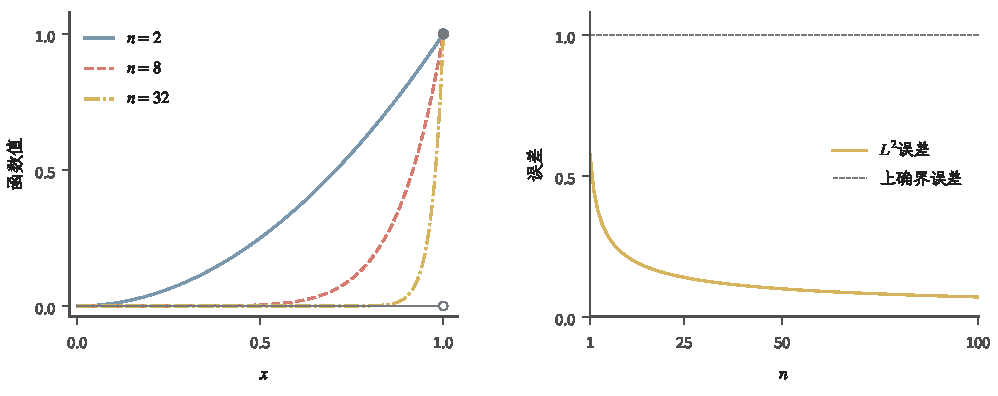
\includegraphics[width=\linewidth]{figures/01-mathematical-preliminaries/01-mathematical-language-combinatorics-analysis-optimization/matplotlib/teaching-analysis/analysis-power-convergence-scales.pdf}
 \caption{$x^n$在$[0,1]$上的两种整体尺度。左图蓝、红、黄线分别取$n=2,8,32$；灰线与端点标记表示逐点极限，
 它在$x<1$处为零、在$x=1$处为$1$。右图黄色曲线为精确的$L^2$误差$(2n+1)^{-1/2}$，
 灰虚线为始终等于$1$的普通上确界误差；单点$x=1$的修改不影响积分。图为解析教学示例。}
 \label{fig:analysis-power-convergence-scales}
\end{figure*}


若$\mu(X)<\infty$且$f_n,f\in L^p$，一致收敛蕴含$L^p$收敛，因为
\[   \lVert f_n-f\rVert_p   \leq   \mu(X)^{1/p}\lVert f_n-f\rVert_{\infty}. \]
当空间测度无穷时，即使各项仍属于$L^p$，这个推论也可能失败。在$\mathbb R$上采用
Lebesgue测度，固定$1\leq p<\infty$，并取
\[
  f_n(x)=\frac1n\mathbb I_{[0,n^p]}(x).
\]
每个$f_n$都属于$L^p$，且$\sup_x|f_n(x)|=1/n\to0$，所以一致收敛到零；但
\[
  \lVert f_n\rVert_p^p=\frac{n^p}{n^p}=1,
\]
因而不在$L^p$中收敛到零。幅度虽降低，非零区域却同步扩大，累计误差没有随之减小。

反过来，积分误差小也不保证整列在几乎每个点收敛。
\begin{example}[小区间轮流扫过定义域]
\label{ex:analysis-lp-without-ae-limit}
在$[0,1)$上按轮次细分区间，令
\[
 f_{2^k+j}(x)=\mathbb I_{[j2^{-k},(j+1)2^{-k})}(x),
 \qquad k=0,1,\ldots,\quad j=0,\ldots,2^k-1.
\]
第$k$轮依次访问$2^k$个小区间，每个函数的$L^p$范数为$2^{-k/p}$，
所以对每个有限$p\geq1$，$f_n\to0$在$L^p$中成立。
但每个$x\in[0,1)$在每轮恰有一次取值$1$，也在无穷多个其他时刻取值$0$。
因此整列在每个$x$处都不收敛。积分看到每次被访问的区间越来越小，
逐点收敛却要求同一个输入从某一时刻起一直稳定，这两个要求不能互代。
\end{example}

普通上确界会被单个异常点改变，而保持可测性的零测集修改不影响积分。
若仍要控制最坏误差，却允许忽略测度为零的例外，就应比较函数绝对值的本质上界。
\begin{definition}[本质有界与绝对值的本质上界]
\label{def:analysis-essential-bound}
设$(X,\mathcal A,\mu)$为测度空间，$f:X\to\mathbb R$可测。其绝对值$|f|$的
\term{本质上确界}（essential supremum）定义为
\[   \operatorname*{ess\,sup}_{x\in X}|f(x)|   =   \inf\{M\geq0:|f(x)|\leq M\text{几乎处处}\}. \]
若集合中没有有限的$M$，上式取$+\infty$；若上式有限，就称$f$本质有界。
这里衡量的是$|f|$的大小，不是一般有符号函数$f$的本质上确界。
\end{definition}

\begin{definition}[$L^\infty$空间与范数]
\label{def:analysis-linfty-space}
在同一测度空间上，$L^\infty(\mu)$由本质有界可测实函数的几乎处处等价类组成，
其范数定义为
\begin{equation}
  \lVert f\rVert_{L^\infty}
  =
  \operatorname*{ess\,sup}_{x\in X}|f(x)|.
\label{eq:analysis-essential-supremum-norm}
\end{equation}
同样用$f$代写等价类$[f]$；该范数不依赖代表元。
\end{definition}
例如在$[0,1]$上使用Lebesgue测度，令$f(0)=100$、其余位置$f(x)=0$，
则普通上确界为$100$，$|f|$的本质上确界却为$0$。
相应地，$\lVert f_n-f\rVert_{L^\infty}\to0$称为$L^\infty$收敛。
对每个$\varepsilon>0$，它要求某个$N$之后的全部误差都在几乎处处意义下
小于$\varepsilon$。可取精度$1/k$，把各$n,k$对应的可测零测例外并为一个零测集$E$；
于是存在同一个$E$，使$f_n$在$X\setminus E$上一致收敛。
反之，这种补集上的一致收敛立即给出$L^\infty$收敛。
因此它蕴含几乎处处收敛，却不一定是原集合上的一致收敛。
上面的$n\mathbb I_{\{0\}}$在$L^\infty$中恒等于零，普通上确界却为$n$。
对$x^n$，本质上确界误差仍为$1$，因为接近$1$的一整段正测度区间保留大误差，
不是删除端点就能消除。

$L^\infty$与有界函数上的普通上确界范数采用不同的对象：普通上确界范数区分
单点修改，$L^\infty$范数忽略的是$\mu$零测集上的修改。对$1\leq p<\infty$，
定义~\ref{def:analysis-lp-space}中的积分表达式满足齐次性和三角不等式，
而几乎处处等价关系保证范数为零时，空间中的元素就是零元素。
这里“范数”指非负、绝对齐次、满足三角不等式且只在零元素上为零的长度函数；
$L^p$的三角不等式及完整空间理论留到第~\ref{chap:functional-analysis-and-approximation}章。
当$0<p<1$时，同一积分表达式仍可用来度量误差大小，但通常不满足三角不等式，
所以不是范数；本章不把这一区间记作范数空间。

一个固定函数序列的一致收敛，讨论的是$n$增大时对所有输入能否共同控制。统计学习中“经验平均一致逼近总体平均”通常还要对候选函数类取上确界，控制对象形如
\[   \sup_{f\in\mathcal{F}}   \left|     \frac1n\sum_{i=1}^nf(X_i)-\int f\,\mathrm{d}P   \right|. \]
这里的一致性针对候选函数$f\in\mathcal{F}$，不是本节式~\eqref{eq:analysis-uniform-convergence}中针对输入$x\in X$的一致收敛。两者都出现上确界，却不能混为同一概念。
其中$X_1,\ldots,X_n$是来自分布$P$的样本，$\mathcal F$是待比较的可积函数类。
逐个$f$找到的样本量要求可以不同；对$\mathcal F$一致则要求一个共同的样本量控制整类函数。

几乎处处和$L^p$范数还依赖所选测度。若$Q$对$P$\term{绝对连续}
（absolutely continuous），记作$Q\ll P$，则原来$P$意义下的零测例外在$Q$下仍可忽略；
也就是对任意可测$A$，$P(A)=0$蕴含$Q(A)=0$。
这一测度关系不等同于前面映射的连续性；概率论中的正式展开见定义~\ref{def:probability-absolute-continuity}。
若没有$Q\ll P$，换分布可能给原零测集正质量。例如$P$是$[0,1]$上的均匀分布，
$Q$把全部质量放在$0$点；两个只在$0$处不同的函数在$P$意义下等价，在$Q$意义下
却可能具有完全不同的误差。
即使$Q\ll P$，$L^p$收敛也不能仅凭零测关系转移。令$P$是$(0,1)$上的长度测度，
$Q(A)=\int_A(2\sqrt x)^{-1}\,\mathrm dx$，其总质量为$1$，并有$Q\ll P$。
固定有限$p\geq1$，取$u_n=n^{1/(2p)}\mathbb I_{(0,1/n)}$，则
\[
 \lVert u_n\rVert_{L^p(P)}^p=n^{-1/2}\to0,\qquad
 \lVert u_n\rVert_{L^p(Q)}^p
 =\sqrt n\int_0^{1/n}\frac{\mathrm dx}{2\sqrt x}=1.
\]
$Q$虽没有给$P$零测集新增质量，却更看重靠近$0$的区域。
若另有统一常数$C$使$Q(A)\leq CP(A)$对所有可测$A$成立，
从简单函数经单调逼近可得$\lVert u\rVert_{L^p(Q)}
\leq C^{1/p}\lVert u\rVert_{L^p(P)}$，
此时才有直接的积分误差转移保证。

\subsubsection{一致柯西列与极限存在}
前面都先给出候选极限，再判断误差；实际构造时可能只知道后面的函数彼此很近。
令$S$为任意非空集合，$\mathcal F_{\mathrm b}(S)$为所有有界实函数$S\to\mathbb{R}$的集合，配备普通上确界范数
\[   \lVert f\rVert_{\infty}   =   \sup_{x\in S}|f(x)|. \]
这里用$\mathcal F_{\mathrm b}(S)$表示有界函数集合，区别于$\mathcal B(X)$表示的Borel集合族。
所比较的是两个函数之间的距离$\lVert f-g\rVert_\infty$，它检查每个输入而不忽略零测例外。
一致柯西条件就是
\[
 \forall\varepsilon>0,\quad\exists N,\quad
 \forall m,n\geq N,\quad\forall x\in S,\quad
 |f_m(x)-f_n(x)|<\varepsilon.
\]
这个空间完备。事实上，若$(f_n)$满足上述条件，对每个固定$x$，
$(f_n(x))$是实柯西列，故存在$f(x)=\lim_n f_n(x)$。
取一个$n_0$使$\lVert f_n-f_{n_0}\rVert_\infty\leq1$对所有充分大的$n$成立，
再令$n\to\infty$，得到$|f(x)|\leq|f_{n_0}(x)|+1$，所以$f$有界。
对任意$\varepsilon>0$，选$N$使$m,n\geq N$时
$\lVert f_m-f_n\rVert_\infty<\varepsilon/2$。固定$n\geq N$并令$m\to\infty$，
对所有$x$都有$|f(x)-f_n(x)|\leq\varepsilon/2$，于是
$\lVert f-f_n\rVert_\infty\leq\varepsilon/2<\varepsilon$。
这证明$f_n$在该空间中收敛到$f$，而不只是分别得到了各个点的极限。

空间$L^\infty$也完备，但其元素是几乎处处等价类，范数是式~\eqref{eq:analysis-essential-supremum-norm}。上面的逐点证明不能原封不动搬过去， 因为不同$n$的代表函数可能各自在不同零测集上修改；严格证明需要先统一这些例外集合。


\subsection{连续性与一致收敛}
前面的完备性说明一致柯西列有函数极限，还可以追问原函数的性质是否保留。
若度量空间$X$上的实函数$f_n$连续，且$f_n$一致收敛到$f$，则$f$连续。
固定$x\in X$与$\varepsilon>0$，先选$n$使$\lVert f-f_n\rVert_\infty<\varepsilon/3$，
再由这个$f_n$在$x$处连续，选$\delta>0$控制
$|f_n(x')-f_n(x)|<\varepsilon/3$。于是$d(x,x')<\delta$时，
\[
 |f(x')-f(x)|
 \leq |f(x')-f_n(x')|+|f_n(x')-f_n(x)|+|f_n(x)-f(x)|
 <\varepsilon.
\]
一致误差同时控制两端，连续性才被保留。仅逐点收敛没有这个共同控制；上面的$x^n$
例子中，各项连续，极限在$x=1$处却不连续。这里回用的是
第~\ref{sec:analysis-local-models}节的连续性，并未使用积分。

一致收敛是这个结论的充分条件，不是极限连续的必要条件。
例如$x^n$在$[0,1)$上的逐点极限恒为零，仍然连续，但其上确界误差始终为$1$。
这不反驳上面的定理，只说明有些不满足统一误差条件的函数列也恰好保留了连续性。

\subsection{求导与极限交换}

连续性保留不意味着变化率也保留。下面的两个反例分别从尖点和振荡说明差别。
用平滑函数
\[   f_{\varepsilon}(x)=\sqrt{x^2+\varepsilon^2},   \qquad \varepsilon>0 \]
逼近$|x|$。由
\[   0\leq f_{\varepsilon}(x)-|x|   =   \frac{\varepsilon^2}   {\sqrt{x^2+\varepsilon^2}+|x|}   \leq\varepsilon, \]
可知$f_{\varepsilon}$在整个$\mathbb{R}$上一致收敛到$|x|$。其导数为
\[   f_{\varepsilon}'(x)   =   \frac{x}{\sqrt{x^2+\varepsilon^2}}. \]
对每个$x\neq0$，导数收敛到$\operatorname{sign}(x)$；在$x=0$处始终为$0$，而$|x|$
在那里没有导数。即使人为规定$\operatorname{sign}(0)=0$，导数收敛也不一致。例如取
$x_\varepsilon=\varepsilon^2>0$，则
\[
  f_\varepsilon'(x_\varepsilon)
  =
  \frac{\varepsilon}{\sqrt{1+\varepsilon^2}}
  \longrightarrow0,
  \qquad
  \operatorname{sign}(x_\varepsilon)=1.
\]
因此两者之差的绝对值趋于$1$，不可能一致收敛。所以函数值的一致逼近不能推出导数的一致逼近。
讨论光滑近似时，必须明确控制的是函数值、导数还是积分误差。
振荡还给出另一个不依赖不可微点的障碍。令
$f_n(x)=\sin(nx)/n$，$x\in[0,2\pi]$，则
$\lVert f_n\rVert_\infty\leq1/n\to0$，但$f_n'(x)=\cos(nx)$不一致趋于零，
甚至在$x=0$始终为$1$。图~\ref{fig:analysis-convergence-obstacles}右侧显示了这种差别。
若目标是近似导数，必须直接控制导数误差或补充保证导数收敛的条件；只增加函数值的精度
并不能消除高频振荡。

若直接控制导数，则可以反过来保证函数与导数一起收敛；还需在一个位置固定函数值，
以免遗漏任意的竖直平移。下面给出闭区间上的一个便于核对的版本。
\begin{theorem}[一致导数逼近与求导保持]
\label{thm:analysis-uniform-derivative-limit}
设$a<b$，$f_n\in C^1([a,b])$。若存在$x_0\in[a,b]$使$f_n(x_0)\to c$，
且$f_n'$在$[a,b]$上一致收敛到$g$，则$f_n$在$[a,b]$上一致收敛到
\[
 f(x)=c+\int_{x_0}^xg(t)\,\mathrm dt.
\]
函数$f$连续，并在$(a,b)$内可微，满足$f'=g$。
\end{theorem}
\begin{proof}
各$f_n'$连续，前面的连续性保持结论说明其一致极限$g$连续。
微积分基本定理给出$f_n(x)=f_n(x_0)+\int_{x_0}^xf_n'(t)\,\mathrm dt$，因此
\[
 \sup_{x\in[a,b]}|f_n(x)-f(x)|
 \leq |f_n(x_0)-c|+(b-a)\lVert f_n'-g\rVert_\infty
 \longrightarrow0.
\]
连续的$g$可积，微积分基本定理又给出内点处$f'(x)=g(x)$。
\end{proof}
定理回用微分与闭区间积分，不需要支配收敛。若不控制$f_n(x_0)$，
$f_n(x)=n$的导数虽恒为零，函数值却没有有限极限；若不控制导数的统一误差，
前面的振荡例子则会阻断求导保持。

\subsection{积分与极限交换}
\label{sec:analysis-limit-integral-interchange}

定义~\ref{def:analysis-pointwise-almost-everywhere-convergence}
和定义~\ref{def:analysis-almost-everywhere-convergence}已经给出逐点与几乎处处收敛。
现在要判断这些位置上的极限能否保留积分这一整体量。
取值于扩展实数的函数列也沿用这一表述；其中趋于$+\infty$或$-\infty$，分别表示
函数值最终超过或低于任意给定的实数阈值。
逐点收敛允许达到同样精度所需的序号随$x$改变；几乎处处收敛还允许在同一个零测集
上没有极限。这两种条件都没有直接控制积分的误差。下面的例子甚至处处收敛，
积分却始终不靠近极限函数的积分。

\subsubsection{积分下界与Fatou引理}

在$(0,1)$上令
\[   f_n(x)=n\mathbb{I}_{(0,1/n)}(x). \]
对每个固定$x>0$，充分大的$n$满足$x\geq1/n$，故$f_n(x)\to0$；然而
\[   \int_0^1f_n(x)\,\mathrm{d}x=1 \]
对所有$n$成立。因此 $\lim_n\int f_n\neq\int\lim_n f_n$。峰越来越窄，却同时越来越高，逐点观察不到被压缩区域中保留下来的总质量。要交换极限与积分，必须阻止这种质量逃逸或集中。
\begin{figure*}[htbp]
 \centering
 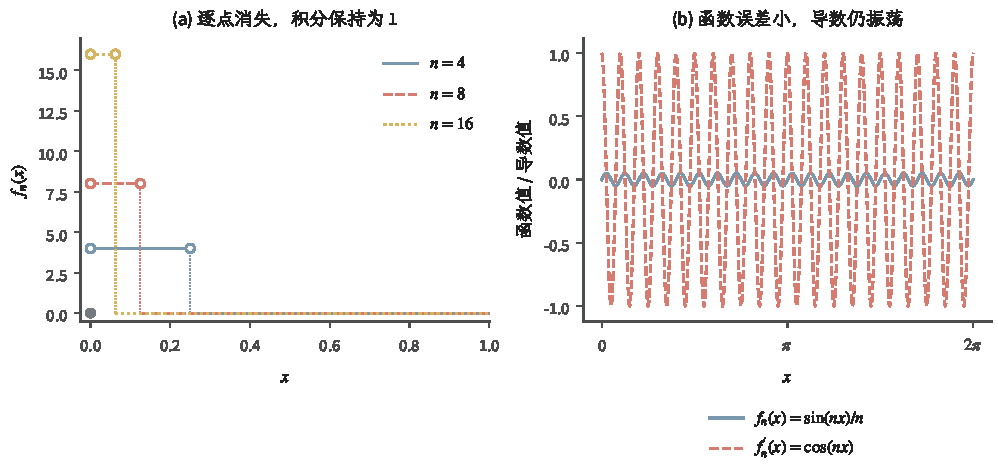
\includegraphics[width=\linewidth]{figures/01-mathematical-preliminaries/01-mathematical-language-combinatorics-analysis-optimization/matplotlib/analysis-geometry/analysis-convergence-obstacles.pdf}
 \caption{两种交换运算的障碍。左图的尖峰支撑不断收缩，但高度同步增长，每条曲线的积分仍为$1$；开圆点标出不取的上端点，竖虚线仅提示跳跃。右图取$n=20$，$\sin(nx)/n$的函数幅度很小，导数$\cos(nx)$仍有单位幅度。两图均为按给定函数公式构造的教学示例。}
 \label{fig:analysis-convergence-obstacles}
\end{figure*}
\FloatBarrier


定理~\ref{thm:analysis-monotone-convergence}已在非负积分构造中证明：非负贡献若逐步
增加，积分便保留其极限。它不要求可积统一上界，也允许无穷总量；现在放宽单调性，
再判断还能得到什么保证。

若只保留非负性，不要求逐步增加，还能得到什么？收缩峰已经说明等式可能失败，
但可以留下一个单向不等式。对不收敛的函数列，回用定义~\ref{def:analysis-liminf-limsup}，在每个$x$处用下极限记录尾部信息。
\begin{lemma}[Fatou引理]
\label{lem:analysis-fatou}
若$f_n:X\to[0,\infty]$可测，则
\begin{equation}
  \int_X\liminf_{n\to\infty}f_n\,\mathrm{d}\mu
  \leq
  \liminf_{n\to\infty}\int_Xf_n\,\mathrm{d}\mu.
\label{eq:analysis-fatou}
\end{equation}
\end{lemma}
\begin{proof}
令$g_n=\inf_{k\geq n}f_k$。则$g_n$可测， $0\leq g_n\uparrow\liminf_k f_k$。由单调收敛定理，
\[   \int\liminf_k f_k\,\mathrm{d}\mu   =   \lim_{n\to\infty}\int g_n\,\mathrm{d}\mu. \]
对每个$k\geq n$都有$g_n\leq f_k$，故
\[   \int g_n\,\mathrm{d}\mu   \leq   \inf_{k\geq n}\int f_k\,\mathrm{d}\mu. \]
令$n\to\infty$便得到式~\eqref{eq:analysis-fatou}。
\end{proof}

Fatou引理通常只给一个方向，因为积分可能在极限中损失质量。对上述收缩峰$f_n$， 左边为$0$，右边为$1$，不等式严格成立。
非负条件也不能直接删除。若改取$u_n=-n\mathbb I_{(0,1/n)}$，则
$\liminf_n u_n=0$处处成立，而$\int u_n=-1$；原不等式会变成错误的$0\leq-1$。
若另有共同的可积下界$h$使$u_n\geq h$，则可以对$u_n-h\geq0$应用Fatou，
再移去有限的$\int h$。可积下界是可用的推广条件，不是无条件允许负值。

\subsubsection{可积支配与积分交换}

若函数会振荡或取负值，单调收敛不适用，Fatou的单向不等式又不足以交换极限。
另一种控制方法是用\emph{同一个可积函数}限制所有逼近的绝对值；它不要求变化单调，
而是阻止越来越高的峰在越来越窄的区域里藏住质量。
\begin{theorem}[支配收敛定理]
\label{thm:analysis-dominated-convergence}
设$f_n,f:X\to\mathbb{R}$可测，$f_n\to f$几乎处处，并且存在非负可积函数$g$使
$|f_n|\leq g$几乎处处对所有$n$成立，则$f$可积，而且
\[   \lim_{n\to\infty}\int_Xf_n\,\mathrm{d}\mu   =   \int_Xf\,\mathrm{d}\mu. \]
此外，$\int|f_n-f|\,\mathrm{d}\mu\to0$。
\end{theorem}
\begin{proof}
把收敛或控制条件失效的可测零测集的可数并记为$N$，并将$f_n,f,g$在$N$上都改为
$0$。这些函数仍可测且积分不变，因而下述关系可以按逐点意义使用。
由$|f_n|\leq g$并取逐点极限可得$|f|\leq g$几乎处处，所以$f$可积。函数$g+f_n$与$g-f_n$均非负。对它们分别使用Fatou引理，
\begin{align*}
  \int g+\int f
  &\leq
  \int g+\liminf_{n\to\infty}\int f_n,\\
  \int g-\int f
  &\leq
  \int g-\limsup_{n\to\infty}\int f_n.
\end{align*}
由于$\int g<\infty$，可以从两边减去它，得到
\[   \int f   \leq\liminf_n\int f_n   \leq\limsup_n\int f_n   \leq\int f. \]
故积分收敛到$\int f$。

最后，$|f_n-f|\to0$几乎处处，且 $|f_n-f|\leq2g$。再对非负函数$|f_n-f|$应用刚证明的积分交换结论，得到 $\int|f_n-f|\,\mathrm{d}\mu\to0$。
\end{proof}

收缩峰$f_n=n\mathbb{I}_{(0,1/n)}$不存在满足条件的可积控制函数。
若$g\geq f_n$几乎处处对每个$n$成立，先把可数个例外集并为$N$。
对$x\in(0,1/4)\setminus N$取$n=\lfloor1/(2x)\rfloor$，
则$n<1/x$且$n\geq1/(4x)$，从而$g(x)\geq f_n(x)=n\geq1/(4x)$。
这个下界在$0$附近不可积，说明失效的是统一可积控制，而不是逐点极限。

贡献还可能逃向无穷远。在$\mathbb R$上取$f_n=\mathbb I_{[n,n+1)}$，
则$f_n\to0$处处成立，积分却恒为$1$。若有共同支配$g$，它须在
$[1,\infty)$上几乎处处至少为$1$，不可能可积。
可积支配同时排除这种向远处移动和前面的局部集中；单纯给出统一常数上界，
在无限测度空间上还不够。

反过来，在$(0,1)$上取$f_n(x)=x^n/\sqrt x$，则逐点趋于零，
且$|f_n|\leq x^{-1/2}$，右侧已知可积。DCT给出$\int f_n\to0$；
直接积分得到$1/(n+1/2)$，核对了结论。支配函数可以无界，
需要有限的是它的积分，而不是普通上确界。

交换符号之前可以按表~\ref{tab:analysis-interchange-conditions}核对实际使用的定理。
“有极限”只提供一个候选函数，附加条件才保证整体量在取极限时被保留下来。

\begin{table*}[htbp]
 \centering\small
 \begin{tabularx}{\linewidth}{@{}lXX@{}}
 \toprule
 结果 & 核对的条件 & 可得到的结论\\
 \midrule
 单调收敛 & 非负可测函数逐点或几乎处处递增 & 极限与积分相等，允许无穷值\\
 Fatou引理 & 非负可测函数列 & 先取下极限再积分，不超过先积分再取下极限的结果\\
 支配收敛 & 几乎处处收敛，且共用一个可积绝对上界 & 积分可交换极限，并有$\int|f_n-f|\,\mathrm d\mu\to0$\\
 Tonelli定理 & $\sigma$有限乘积测度上的非负可测函数 & 交换积分次序，允许无穷值\\
 Fubini定理 & $\sigma$有限乘积测度上的绝对可积函数 & 交换积分次序，并得到有限积分\\
 \bottomrule
 \end{tabularx}
 \caption{极限与积分、积分与积分之间的交换条件。表中的测度、可测性和统一控制属于结论的假设。}
 \label{tab:analysis-interchange-conditions}
\end{table*}

\subsubsection{参数求导与积分交换}

给定参数以后，$g(\cdot,\theta)$是一个函数；让参数接近$\theta_0$时，差商形成一族
逼近函数。因此积分号下求导同时使用第~\ref{sec:analysis-local-models}节的微分、
第~\ref{sec:analysis-integration-average}节的积分，以及刚证明的支配收敛，不能只由
各点偏导数存在就交换运算。


设
\[   G(\theta)=\int_X g(x,\theta)\,\mathrm{d}\mu(x). \]
形式上希望把导数移入积分号：
\[   G'(\theta)   \stackrel{?}{=}   \int_X\frac{\partial g}{\partial\theta}(x,\theta)\,\mathrm{d}\mu(x). \]
真正需要交换的是差商的极限与积分。固定$\theta_0$，设对每个$\theta\in I$，
$x\mapsto g(x,\theta)$可测，其中$I$是包含$\theta_0$的开区间，并且
$g(\cdot,\theta_0)$可积。假设存在一个可测零测集$N$，使每个$x\notin N$处的
$\theta\mapsto g(x,\theta)$在整个$I$内可微；对每个$\theta$，
偏导数作为$x$的函数可测，并且存在非负可积函数$h$使
\begin{equation}
  \left|
    \frac{\partial g}{\partial\theta}(x,\theta)
  \right|
  \leq h(x)
  \quad
  \text{对所有$x\notin N$及所有$\theta\in I$成立},
\label{eq:analysis-parameter-derivative-domination}
\end{equation}
这里$N$和$h$都不能随参数$\theta$改变；参数不可数，不能靠取所有参数例外集的并
自动获得一个零测集。中值定理先给出
$|g(x,\theta)-g(x,\theta_0)|\leq|\theta-\theta_0|h(x)$，
所以$I$中每个$g(\cdot,\theta)$都可积，$G$在邻域内有有限值。
对非零$t$且$\theta_0+t\in I$，令
\[
 q_t(x)=\frac{g(x,\theta_0+t)-g(x,\theta_0)}{t}.
\]
中值定理又给出$|q_t(x)|\leq h(x)$于$X\setminus N$。
差商在那里趋于$\partial g/\partial\theta(x,\theta_0)$。
对任意非零序列$t_n\to0$应用支配收敛，得到同一个积分极限；
由实数极限的序列判据，这就是$t\to0$的双侧极限。因此
\begin{equation}
  G'(\theta_0)
  =
  \int_X
  \frac{\partial g}{\partial\theta}(x,\theta_0)
  \,\mathrm{d}\mu(x).
\label{eq:analysis-differentiate-under-integral}
\end{equation}
条件~\eqref{eq:analysis-parameter-derivative-domination}是一个便于核对的充分条件； 更一般的版本可以直接控制差商，或使用其他一致可积条件。

例如令$g(x,\theta)=e^{-\theta x}$，$x\in[0,\infty)$、$\theta>0$，
并用Lebesgue测度积分。固定$\theta_0>0$后取
$I=(\theta_0/2,3\theta_0/2)$，则
$|\partial_\theta g|=xe^{-\theta x}\leq xe^{-\theta_0x/2}=:h(x)$。
分部积分给出$\int_0^\infty h(x)\,\mathrm dx=4/\theta_0^2<\infty$，
没有需要删除的例外点，故
$G'(\theta_0)=-\int_0^\infty xe^{-\theta_0x}\,\mathrm dx=-1/\theta_0^2$，
与$G(\theta)=1/\theta$的直接求导一致。
若把参数范围放大到任意接近零的正数，便不能沿用这个固定的控制函数；
交换结论所需的是所考察参数点附近的统一控制。

\begin{example}[参数积分中的控制函数失效]
\label{ex:analysis-parameter-integral-failure}
下面考察参数域边界处对应的右求导问题。对$\theta\geq0$与$x\in(0,1)$，定义
\[   g(x,\theta)   =
\begin{cases}     \dfrac{\theta x}{x^2+\theta^2}, & \theta>0,\\[5pt]     0, & \theta=0.
\end{cases} \]
每个固定$x>0$处关于$\theta$的右偏导数都等于$1/x$，但$1/x$在$(0,1)$上不可积。
直接积分得到
\[   G(\theta)   =   \frac{\theta}{2}   \log\left(\frac{1+\theta^2}{\theta^2}\right)   \quad(\theta>0),   \qquad G(0)=0. \]
于是$G(\theta)/\theta$在$\theta\downarrow0$时发散，$G$在$0$处没有有限右导数。积分内的
逐点右导数虽然存在，却缺少统一可积控制；因此这里不能交换右求导与积分。
\end{example}

\section{本章小结}
\label{sec:analysis-summary}

无限过程需要同时说明对象、结构与控制条件。距离比较点与点，测度为集合赋权，
二者分别决定收敛与累计的含义。测度完备化处理零测集的子集，度量完备性保证柯西
点列的极限留在空间内；它们承担不同职责。部分和和更新迭代都产生序列，单步误差
趋零不能替代尾和控制，而统一压缩把几何尾和落实为解的存在、唯一和停止误差。

固定一个函数以后，连续性控制输入扰动，微分提供局部线性模型，二阶信息与Taylor
余项说明曲率及近似损失。隐函数定理把方程的局部解建立为可微函数，使解导数与
最优值的包络导数能够区分。尖点、跳跃和替代更新信号又说明，真实导数、广义梯度
与人为指定的反向信号必须分别判断。

整体累计依赖可测范围和权重。简单函数把积分还原为有限贡献，单调逼近进入一般
非负函数，绝对可积性排除正负无穷相消；积分只有在总权重为$1$或完成归一化后才是
平均。乘积测度、换元与边界公式各自改变累计的对象或表示，积分次序、体积修正与
边界项都有明确条件，不能由有限和的操作习惯直接代替。

函数列仍是序列，但逐点、一致与积分误差控制不同内容。统一逼近能够保留连续性，
却不自动保留导数；非负单调性或共同可积支配则控制极限与积分的关系。积分号下求导
把这两条线结合起来：差商必须既趋向导数，又有足够的积分控制。后续使用这些工具时，
应先辨认当前对象及所需保证，再核对定义域、光滑性、可积性与统一条件。
第~\ref{chap:optimization}章据此研究最优性与求解，第~\ref{chap:functional-analysis-and-approximation}章
进一步研究函数空间中的表示、逼近和稳定性。
